\documentclass[
twoside,
%draft,           %use this for fast draft compilation with additional overfull boxes hint bars (also affects graphicx)
a4paper,          %A4 paper size
11pt,             %well readable for A4 printing
numbers=noenddot, %no trailing dot after numbers for chapters, sections, etc.
cleardoublepage=empty, %nice left plain pages before chapters
%chapterprefix,    %chapter X prefix before chapters
%appendixprefix,   %appendix X prefix before appendices
headsepline,      %lines in header
%headtopline,      %lines in header
footbotline,      %lines in footer
%footsepline,      %lines in footer
plainfootbotline, %lines in footer for scrplain page style
%plainfootsepline, %lines in footer for srcplain page style
%ilines,
DIV=15,            %adjust this value for more/less text on pages
BCOR=5mm % binding correction
]{scrbook}

%%%packages
\usepackage[]{scrpage2} %%% koma script for nice layout
\usepackage[english,ngerman]{babel}   %%% an english thesis usually has a german synopsis
%\usepackage[T1]{fontenc}      %%%this lets you use äöüß instead of \"a \ss{} etc....
\usepackage[latin1]{inputenc}  %%%...which makes german tex files
\usepackage[numbers,square,comma,sort&compress]{natbib}
\bibliographystyle{unsrtnatMod}
\usepackage[absolute,overlay]{textpos} %textblock env for text positioning
\usepackage{multirow}
\usepackage{amsmath} %Zus�tzliches Mathepaket, dass die Align-Umgebung beinhaltet
\usepackage{amsfonts} %%% math fonts needed
\usepackage{amssymb}  %%% maths symbols needed 
\usepackage{bm}
\usepackage{physics} 
\usepackage{xcolor}
\usepackage{float}
\usepackage{graphicx}
\usepackage{tabularx}
\graphicspath{{figure/}} 
\usepackage{wrapfig}
\usepackage{rotating}
\usepackage{caption}
\usepackage{subcaption}
\usepackage{units}
\usepackage[breaklinks=true]{hyperref}
\usepackage{helvet}
\usepackage{titlesec}
%\usepackage[hyperpageref]{backref}
\usepackage[draft]{todonotes}   % draft: notes showed, disable: not showed
\usepackage{comment}
%\renewcommand{\comment}[1]{}  %comment not showed
\renewcommand{\comment}[1] {\par {\bfseries \color{blue} #1 \par}} %comment showed
\usepackage{epstopdf}
\usepackage{dsfont}
\usepackage{lipsum}
%%%%macros
%macro file 
\newcommand{\trm}[1]{\textrm{#1}} 
\newcommand{\e}[1]{\cdot 10^{#1}} 
\newcommand{\mc}[1]{\mathcal{#1}}
\newcommand{\tbf}[1]{\textbf{#1}}
\newcommand{\ttt}[1]{\texttt{#1}}
\newcommand{\mal}[1]{\begin{align}#1 \end{align}}
\newcommand{\malnotag}[1]{\begin{align}#1\end{align}}
\newcommand{\ol}[1]{\bar{#1}}
\newcommand{\pic}[3]{ \begin{figure}[H] \centering \includegraphics[width=#2\linewidth]{pics/#1} \caption{#3} \label{fig:#1} \end{figure}}
\newcommand{\mb}[1]{\mathbf{#1}}
\newcommand{\red}[1]{\textcolor{red}{#1}}
\newcommand{\green}[1]{\textcolor{green}{#1}}
\newcommand{\blue}[1]{\textcolor{blue}{#1}}
\newcommand{\da}{^{\dagger}}
\newcommand{\up}{\uparrow}
\newcommand{\down}{\downarrow}
\newcommand{\T}{^{\trm{T}}}
\newcommand{\icdw}{\trm{iCDW}}
\newcommand{\sdw}{\trm{SDW}}
\newcommand{\rpa}{\trm{RPA}}
\newcommand{\Abs}[1]{\abs{#1}}
\newcommand{\inter}{\trm{inter}}
\newcommand{\intra}{\trm{intra}}
\newcommand{\om}{\tilde{\omega}}
\newcommand{\ti}[1]{\tilde{#1}}
\newcommand{\res}{\trm{Res}}
\newcommand{\circeld}[2]{\raisebox{0.5pt}{\textcircled{\raisebox{-#2pt} {#1}}}}
\newcommand{\circeldF}{\circeld{f}{1.5}}
\newcommand{\circeldC}{\circeld{c}{0.}}
\newcommand{\bk}{\mb{k}}
\newcommand{\br}{\mb{r}}
\newcommand{\bq}{\mb{q}}
\newcommand{\hc}{\trm{h.c.}}
\newcommand{\bQx}{\mb{Q}_{x}}
\newcommand{\cfbox}[2]{%
    \colorlet{currentcolor}{.}%
    {\color{#1}%
    \fbox{\color{currentcolor}#2}}%
}

% box
\newcommand{\textbox}[2]{\centering \textcolor{KITblack30}{\shadowbox{\parbox{#1\columnwidth}{\centering \textcolor{KITblack}{\\ \textit{#2}}}}}}

\newcommand{\capt}[1]{\textcolor{KITblack50}{\small #1}}

\newcommand{\Justify}{\justify\vspace{-1cm}}

%%%layout
%%%%
%own
%%%%

%%%%%%%%%%%%%%%%%%%%%%%%%%%%%%
%%Globale Layouteinstellungen%
%%%%%%%%%%%%%%%%%%%%%%%%%%%%%%
%%%at uni
% % %for page size and margin see https://www.sharelatex.com/learn/Page_size_and_margins
\setlength{\headheight}{0cm}              % H�he der Kopfzeile
\setlength{\textheight}{23.5cm}              % Texth�he

%%%at home
%\setlength{\headheight}{1.5cm}              % H�he der Kopfzeile
%\setlength{\textheight}{23.0cm}              % Texth�he
%\setlength{\footskip}{1cm}

%\setlength{\textwidth}{16.0cm}               % Textbreite
%\setlength{\topmargin}{1.0cm}               % oberen Seitenrand festlegen, bzw. verschieben
%\setlength{\oddsidemargin}{0.2cm}            % Seitenrand anpassen -> ungerade Seiten !
%\setlength{\evensidemargin}{-0.2cm}          % Seitenrand anpassen -> gerade Seiten !
%\setcounter{secnumdepth}{5}                  % Schachtelungstiefe Ueberschriften
%\setcounter{tocdepth}{5}                     % Schachtelungstiefe Eintraege im Inhaltsverzeichnis
%\setlength{\parindent}{0pt}                  % Einzug bei neuen Abs�tzen
%\setlength{\parskip}{5pt plus 2pt minus 1pt} % Abstand zwischen zwei Abs�tzen
%\renewcommand{\baselinestretch}{1.1}         % Ver�nderung des Zeilenabstandes {Faktor}

%%%%%%%%%%%%%%%%%%%%%%%%%%%%%% 
%%Globale Headingeinsellungen and spacing before and after headings%
%%%%%%%%%%%%%%%%%%%%%%%%%%%%%%
%\titleformat{\chapter}[hang]{\Large\bfseries}{\thechapter}{5pt}{} % changes font of chapter 
%\titlespacing{\chapter} % changes spacing 
%{0pc}{*3}{*1}[0pc]
%\titlespacing{\section}
%{0pc}{*2}{*1}[0pc]
%\titlespacing{\subsection}
%{0pc}{*2}{*1}[0pc]
%\titlespacing{\subsubsection}
%{0pc}{*0}{*0}[0pc]

%%%%%%%%%%%%%%%%%%%%%%%%%%%%%%%%%%%%%%%%%%%%
%Eigene Einstellungen zu Fu�- und Kopfzeile%
%%%%%%%%%%%%%%%%%%%%%%%%%%%%%%%%%%%%%%%%%%%%
%\usepackage{fancyhdr}
%\pagestyle{fancy}
%\renewcommand{\chaptermark}[1]{\markboth{#1}{}} 	%Modifizierung des Befehls \leftmark
%\renewcommand{\sectionmark}[1]{\markright{#1}{}}	%Modifizierung des Befehls \rightmark
%\fancyhf{} 										%alle Kopf- und Fu�zeilenfelder bereinigen
%\fancyhead[L]{\chaptername} 	%Kopfzeile links :\leftmark: Kapitel, :\rightmark: Unterkapitel
%\fancyhead[C]{}								%zentrierte Kopfzeile
%\fancyhead[R]{\leftmark} 			%Kopfzeile rechts
%\renewcommand{\headrulewidth}{0.4pt} %obere Trennlinie
%\fancyfoot[C]{\thepage} 			%Seitennummer
%\renewcommand{\footrulewidth}{0.4pt} %untere Trennlinie%\pagestyle{fancy}
%\renewcommand{\chaptermark}[1]{\markboth{#1}{}} 	%Modifizierung des Befehls \leftmark
%\renewcommand{\sectionmark}[1]{\markright{#1}{}}	%Modifizierung des Befehls \rightmark
%\fancyhf{} 										%alle Kopf- und Fu�zeilenfelder bereinigen
%\fancyhead[L]{\chaptername} 	%Kopfzeile links :\leftmark: Kapitel, :\rightmark: Unterkapitel
%\fancyhead[C]{}								%zentrierte Kopfzeile
%\fancyhead[R]{\leftmark} 			%Kopfzeile rechts
%\renewcommand{\headrulewidth}{0.4pt} %obere Trennlinie
%\fancyfoot[C]{\thepage} 			%Seitennummer
%\renewcommand{\footrulewidth}{0.4pt} %untere Trennlinie

%\makeindex %erstellt ein Stichwortindex

%%%%%
%space before and after figure envr
%%%%%
%\setcounter{topnumber}{2}
%\setcounter{bottomnumber}{2}
%\setcounter{totalnumber}{4}
%\renewcommand{\topfraction}{0.85}
%\renewcommand{\bottomfraction}{0.85}
%\renewcommand{\textfraction}{0.15}
%\renewcommand{\floatpagefraction}{0.8}
%\renewcommand{\textfraction}{0.1}
%\setlength{\floatsep}{5pt plus 2pt minus 2pt}
%\setlength{\textfloatsep}{5pt plus 2pt minus 2pt}
%\setlength{\intextsep}{5pt plus 2pt minus 2pt}

%%%%
%von Pi
%%%%

%%% A bugfix regarding transparency in PDF viewers
%%% I have no idea what this command does...
\pdfpageattr{/Group << /S /Transparency /I true /CS /DeviceRGB>>} 

%%%%%%%%%%%%%%%%%%%%%%%%%%%%%%%%%%%%%%%%%%%%%%%%%%
%%% description label font
%%%%%%%%%%%%%%%%%%%%%%%%%%%%%%%%%%%%%%%%%%%%%%%%%%
%%% When using helvetic as font, the description labels become to
%%% large, so let's use the standard text font and make it bold (which
%%% i like better anyways...)
\setkomafont{descriptionlabel}{\normalfont\bfseries} % labels, i. e., the optional argument of \item in the description environment (see section 3.18, page 106)

%%%%%%%%%%%%%%%%%%%%%%%%%%%%%%%%%%%%%%%%%%%%%%%%%%
%%% hyperlinks and bookmarks menu for online reading
%%%%%%%%%%%%%%%%%%%%%%%%%%%%%%%%%%%%%%%%%%%%%%%%%%
\hypersetup{bookmarksopen=true,
bookmarksnumbered=true}
\definecolor{my_red}{rgb}{0.5,0,0}
\definecolor{my_green}{rgb}{0,0.5,0}
\definecolor{my_blue}{rgb}{0,0,0.5}
\hypersetup{
        pdftitle={the title},
        pdfauthor={the author},
        pdfsubject={Diploma Thesis},
        pdfkeywords={the keywords},
        pdfborder=000,
        colorlinks=false,
        urlcolor=my_red,
        linkcolor=my_blue,
        citecolor=my_green,
        pdfpagemode=UseNone,
        plainpages=false,
        bookmarksopen=true,
        final=true
}

%\renewcommand*{\backref}[1]{}
%\renewcommand*{\backrefalt}[4]{\\\mbox{\small\ifcase #1 (Not cited.) \or
%(Cited on page #2.) \else (Cited on pages #2.)\fi}} 

%% general unit is 1 cm
%\setlength{\unitlength}{1cm}

%%%%%%%%%%%%%%%%%%%%%%%%%%%%%%%%%%%%%%%%%%%%%%%%%%
%%% the abstract before each chapter telling the reader
%%% what will be described here
%%%%%%%%%%%%%%%%%%%%%%%%%%%%%%%%%%%%%%%%%%%%%%%%%%
\newenvironment{chapterabstract}{\itshape}{}

%%%%%%%%%%%%%%%%%%%%%%%%%%%%%%%%%%%%%%%%%%%%%%%%%%
%%% layout for caption and captionlabels
%%%%%%%%%%%%%%%%%%%%%%%%%%%%%%%%%%%%%%%%%%%%%%%%%%
\renewcommand{\captionfont}{\itshape}
\renewcommand{\captionlabelfont}{\bfseries \upshape}
\setlength{\captionmargin}{10pt}
\captionsetup{
  format=plain,
  margin=0em,
%  labelsep=newline,
%  justification=raggedright
}

%%%%%%%%%%%%%%%%%%%%%%%%%%%%%%%%%%%%%%%%%%%%%%%%%%
%%% a general purpose width, set where needed and
%%% helps typesetting mainly math equations where
%%% equal box sizes are needed
%%%%%%%%%%%%%%%%%%%%%%%%%%%%%%%%%%%%%%%%%%%%%%%%%%
%\newlength{\auxwidth} 

%%%%%%%%%%%%%%%%%%%%%%%%%%%%%%%%%%%%%%%%%%%%%%%%%%
%%% width for mode pictures,
%%% which will be set side by side. this width is
%%% set when needed
%%%%%%%%%%%%%%%%%%%%%%%%%%%%%%%%%%%%%%%%%%%%%%%%%%
%\newlength{\modewidth} 

%%%%%%%%%%%%%%%%%%%%%%%%%%%%%%%%%%%%%%%%%%%%%%%%%%
%%% separator line widths
%%%%%%%%%%%%%%%%%%%%%%%%%%%%%%%%%%%%%%%%%%%%%%%%%%
%\setheadtopline{2pt}
\setheadsepline{0.4pt} %thickness
%\setfootsepline{0.5pt}
\setfootbotline{0.4pt}

\delimitershortfall=-2pt

%%%%%%%%%%%%%%%%%%%%%%%%%%%%%%%%%%%%%%%%%%%%%%%%%%%
%%%% width for one, two, three, four plots per line
%%%%%%%%%%%%%%%%%%%%%%%%%%%%%%%%%%%%%%%%%%%%%%%%%%%
%\newlength{\thisplotwidth}
%
%\newlength{\plotwidthOne} 
%\setlength{\plotwidthOne}{0.975\textwidth} 
%\newlength{\plotwidthTwo} 
%\setlength{\plotwidthTwo}{0.477\textwidth} 
%\newlength{\plotwidthThree} 
%\setlength{\plotwidthThree}{0.31\textwidth} 
%\newlength{\plotwidthThreeTwo} 
%\setlength{\plotwidthThreeTwo}{0.642\textwidth} 
%\newlength{\plotwidthThreeOne} 
%\setlength{\plotwidthThreeOne}{0.31\textwidth} 
%\newlength{\plotwidthFour} 
%\setlength{\plotwidthFour}{0.227\textwidth} 
%
%\newcommand{\includeannotatedplot}[3]{
%  \parbox{#1}{
%    \centering    
%    \includegraphics[width=#1]{#2}\\
%    #3
%  }
%}

%%%%%%%%%%%%%%%%%%%%%%%%%%%%%%%%%%%%%%%%%%%%%%%%%%%%%%%%%%%%
%%%%%%%%%%%%%%%%%%%%%%%%%%%%%%%%%%%%%%%%%%%%%%%%%%%%%%%%%%%%
%%%%%%%                            %%%%%%%%%%%%%%%%%%%%%%%%%
%%%%%   color definitions            %%%%%%%%%%%%%%%%%%%%%%%
%%%%%%                             %%%%%%%%%%%%%%%%%%%%%%%%%
%%%%%%%%%%%%%%%%%%%%%%%%%%%%%%%%%%%%%%%%%%%%%%%%%%%%%%%%%%%%
%%%%%%%%%%%%%%%%%%%%%%%%%%%%%%%%%%%%%%%%%%%%%%%%%%%%%%%%%%%%
\definecolor{greenyellow}   {cmyk}{0.15, 0   , 0.69, 0   }
\definecolor{yellow}        {cmyk}{0   , 0   , 1   , 0   }
\definecolor{goldenrod}     {cmyk}{0   , 0.10, 0.84, 0   }
\definecolor{dandelion}     {cmyk}{0   , 0.29, 0.84, 0   }
\definecolor{apricot}       {cmyk}{0   , 0.32, 0.52, 0   }
\definecolor{peach}         {cmyk}{0   , 0.50, 0.70, 0   }
\definecolor{melon}         {cmyk}{0   , 0.46, 0.50, 0   }
\definecolor{yelloworange}  {cmyk}{0   , 0.42, 1   , 0   }
\definecolor{orange}        {cmyk}{0   , 0.61, 0.87, 0   }
\definecolor{burntorange}   {cmyk}{0   , 0.51, 1   , 0   }
\definecolor{bittersweet}   {cmyk}{0   , 0.75, 1   , 0.24}
\definecolor{redorange}     {cmyk}{0   , 0.77, 0.87, 0   }
\definecolor{mahogany}      {cmyk}{0   , 0.85, 0.87, 0.35}
\definecolor{maroon}        {cmyk}{0   , 0.87, 0.68, 0.32}
\definecolor{brickred}      {cmyk}{0   , 0.89, 0.94, 0.28}
\definecolor{red}           {cmyk}{0   , 1   , 1   , 0   }
\definecolor{orangered}     {cmyk}{0   , 1   , 0.50, 0   }
\definecolor{rubinered}     {cmyk}{0   , 1   , 0.13, 0   }
\definecolor{wildstrawberry}{cmyk}{0   , 0.96, 0.39, 0   }
\definecolor{salmon}        {cmyk}{0   , 0.53, 0.38, 0   }
\definecolor{carnationpink} {cmyk}{0   , 0.63, 0   , 0   }
\definecolor{magenta}       {cmyk}{0   , 1   , 0   , 0   }
\definecolor{violetred}     {cmyk}{0   , 0.81, 0   , 0   }
\definecolor{rhodamine}     {cmyk}{0   , 0.82, 0   , 0   }
\definecolor{mulberry}      {cmyk}{0.34, 0.90, 0   , 0.02}
\definecolor{redviolet}     {cmyk}{0.07, 0.90, 0   , 0.34}
\definecolor{fuchsia}       {cmyk}{0.47, 0.91, 0   , 0.08}
\definecolor{lavender}      {cmyk}{0   , 0.48, 0   , 0   }
\definecolor{thistle}       {cmyk}{0.12, 0.59, 0   , 0   }
\definecolor{orchid}        {cmyk}{0.32, 0.64, 0   , 0   }
\definecolor{darkorchid}    {cmyk}{0.40, 0.80, 0.20, 0   }
\definecolor{purple}        {cmyk}{0.45, 0.86, 0   , 0   }
\definecolor{plum}          {cmyk}{0.50, 1   , 0   , 0   }
\definecolor{violet}        {cmyk}{0.79, 0.88, 0   , 0   }
\definecolor{royalpurple}   {cmyk}{0.75, 0.90, 0   , 0   }
\definecolor{blueviolet}    {cmyk}{0.86, 0.91, 0   , 0.04}
\definecolor{periwinkle}    {cmyk}{0.57, 0.55, 0   , 0   }
\xdefinecolor{cadetblue}     {cmyk}{0.62, 0.57, 0.23, 0   }
\xdefinecolor{cornflowerblue}{cmyk}{0.65, 0.13, 0   , 0   }
\xdefinecolor{midnightblue}  {cmyk}{0.98, 0.13, 0   , 0.43}
\xdefinecolor{navyblue}      {cmyk}{0.94, 0.54, 0   , 0   }
\xdefinecolor{royalblue}     {cmyk}{1   , 0.50, 0   , 0   }
\definecolor{blue}          {cmyk}{1   , 1   , 0   , 0   }
\xdefinecolor{darkblue}     {cmyk}{1   , 1   , 0   , 0.5 }
\definecolor{cerulean}      {cmyk}{0.94, 0.11, 0   , 0   }
\definecolor{cyan}          {cmyk}{1   , 0   , 0   , 0   }
\definecolor{processblue}   {cmyk}{0.96, 0   , 0   , 0   }
\definecolor{skyblue}       {cmyk}{0.62, 0   , 0.12, 0   }
\definecolor{turquoise}     {cmyk}{0.85, 0   , 0.20, 0   }
\definecolor{tealblue}      {cmyk}{0.86, 0   , 0.34, 0.02}
\definecolor{aquamarine}    {cmyk}{0.82, 0   , 0.30, 0   }
\definecolor{bluegreen}     {cmyk}{0.85, 0   , 0.33, 0   }
\definecolor{emerald}       {cmyk}{1   , 0   , 0.50, 0   }
\definecolor{junglegreen}   {cmyk}{0.99, 0   , 0.52, 0   }
\definecolor{seagreen}      {cmyk}{0.69, 0   , 0.50, 0   }
\definecolor{green}         {cmyk}{1   , 0   , 1   , 0   }
\definecolor{forestgreen}   {cmyk}{0.91, 0   , 0.88, 0.12}
\definecolor{pinegreen}     {cmyk}{0.92, 0   , 0.59, 0.25}
\definecolor{limegreen}     {cmyk}{0.50, 0   , 1   , 0   }
\definecolor{yellowgreen}   {cmyk}{0.44, 0   , 0.74, 0   }
\definecolor{springgreen}   {cmyk}{0.26, 0   , 0.76, 0   }
\definecolor{olivegreen}    {cmyk}{0.64, 0   , 0.95, 0.40}
\definecolor{rawsienna}     {cmyk}{0   , 0.72, 1   , 0.45}
\definecolor{sepia}         {cmyk}{0   , 0.83, 1   , 0.70}
\definecolor{brown}         {cmyk}{0   , 0.81, 1   , 0.60}
\definecolor{tan}           {cmyk}{0.14, 0.42, 0.56, 0   }
\definecolor{gray}          {cmyk}{0   , 0   , 0   , 0.50}
\definecolor{black}         {cmyk}{0   , 0   , 0   , 1   }
\definecolor{white}         {cmyk}{0   , 0   , 0   , 0   } 
\definecolor{darkgray}      {cmyk}{0   , 0   , 0   , 0.75}

%%% end of chapter headings
%%%%%%%%%%%%%%%%%%%%%%%%%%%%%%%%%%%%%%%%%%%%%%%%%%%%%%%%%%%%
%%%%%%%%%%%%%%%%%%%%%%%%%%%%%%%%%%%%%%%%%%%%%%%%%%%%%%%%%%%%



%%%%%%%%%%%%%%%%%%%%%%%%%%%%%%%%%%%%%%%%%%%%%%%%%%%%%%%%%%%%
%%%%%%%%%%%%%%%%%%%%%%%%%%%%%%%%%%%%%%%%%%%%%%%%%%%%%%%%%%%%
%%%%%%%                            %%%%%%%%%%%%%%%%%%%%%%%%%
%%%%%   boxed equations             %%%%%%%%%%%%%%%%%%%%%%%
%%%%%%                             %%%%%%%%%%%%%%%%%%%%%%%%%
%%%%%%%%%%%%%%%%%%%%%%%%%%%%%%%%%%%%%%%%%%%%%%%%%%%%%%%%%%%%
%%%%%%%%%%%%%%%%%%%%%%%%%%%%%%%%%%%%%%%%%%%%%%%%%%%%%%%%%%%%

%%%%%%%%%%%%%%%%%%%%%%%%%%%%%%%%%%%%%%%%%%%%%%%%%%
%%% create boxed formulas within a math environment
%%% newlines are allowed in the source
%%% (this is not the case when using the AMS command \boxed)
%%%%%%%%%%%%%%%%%%%%%%%%%%%%%%%%%%%%%%%%%%%%%%%%%%
%\newcommand{\mathbox}[1]{
%    \fbox{ $ \displaystyle #1 $ }
%}
%
%%%%
%\newcommand*\widefbox[1]{\fbox{\hspace{1em}#1\hspace{1em}}}
%
%%%% Simple box containing subequations
%\newcommand*{\boxedsubeq}[2]{%
%\begin{subequations}\label{#1}%
%\begin{empheq}[box=\widefbox]{align}%
%#2
%\end{empheq}%
%\end{subequations}
%}
%
%%%% Very fancy box containing subequations
%\definecolor{shadecolor}{cmyk}{0,0,0.21,0}%
%\definecolor{headercolor}{cmyk}{0,0,0.5,0}%{0.25,0,0,0}
%%\colorlet{shadecolor}{gray}
%
%\newsavebox{\mysaveboxM}
%\newsavebox{\mysaveboxT}
%
%\newcommand*{\fancyBoxedSubeq}[2][Example]{%
% \sbox{\mysaveboxM}{#2}%
% \sbox{\mysaveboxT}{\fcolorbox{black}{headercolor}{#1}}%
% \sbox{\mysaveboxM}{%
%  \parbox[b][\ht\mysaveboxM+.5\ht\mysaveboxT+.5\dp\mysaveboxT][b]{%
%    \wd\mysaveboxM}{#2}%
% }%
%\sbox{\mysaveboxM}{%
%  \fcolorbox{black}{shadecolor}{%
%     \makebox[\linewidth-5em]{\usebox{\mysaveboxM}}%
%  }%
% }%
%  \usebox{\mysaveboxM}%
%  \makebox[0pt][r]{%
%    \makebox[\wd\mysaveboxM][c]{%
%       \raisebox{\ht\mysaveboxM-0.5\ht\mysaveboxT
%                 +0.5\dp\mysaveboxT-0.5\fboxrule}{\usebox{\mysaveboxT}}%
%    }%
%  }%
%}

%%%%%%%%%%%%%%%%%%%%%%%%%%%%%%%%%%%%%%%%%%%%%%%%%%%%%%%%%%%%
%%%%%%%%%%%%%%%%%%%%%%%%%%%%%%%%%%%%%%%%%%%%%%%%%%%%%%%%%%%%
%%%%%%%                            %%%%%%%%%%%%%%%%%%%%%%%%%
%%%%%   chapter headings             %%%%%%%%%%%%%%%%%%%%%%%
%%%%%%                             %%%%%%%%%%%%%%%%%%%%%%%%%
%%%%%%%%%%%%%%%%%%%%%%%%%%%%%%%%%%%%%%%%%%%%%%%%%%%%%%%%%%%%
%%%%%%%%%%%%%%%%%%%%%%%%%%%%%%%%%%%%%%%%%%%%%%%%%%%%%%%%%%%%

%%% INFO: when using different fonts, the chapter headings may look
%%% different and the given sizes do no longer apply!

\colorlet{chapter}{darkblue}
\addtokomafont{chapter}{\color{black}}

\makeatletter% siehe De-TeX-FAQ
\renewcommand*{\chapterformat}{%
\begingroup% damit \unitlength-Änderung lokal bleibt
\setlength{\unitlength}{1mm}%
\begin{picture}(20,40)(0,5)%
\setlength{\fboxsep}{0pt}%
%\put(0,0){\framebox(20,30){}}%
%\put(0,20){\makebox(20,20){\rule{20\unitlength}{20\unitlength}}}%
\put(20,15){\color{black}\linethickness{0.4pt}\line(1,0){\dimexpr\textwidth-20\unitlength\relax\@gobble}}% line
\put(0,0){\makebox(18,20)[r]{\fontsize{20\unitlength}{1}\color{black}\selectfont\thechapter %\kern-.04em% Ziffer in der Zeichenzelle nach rechts schieben
}}%
\put(20,15){\makebox(\dimexpr \textwidth-20\unitlength\relax\@gobble,\ht\strutbox\@gobble)[l]{%\ %\normalsize\color{black}\chapapp~\thechapter\autodot 
}}%
\end{picture} % <- Leerzeichen ist hier beabsichtigt!
\endgroup
}%
\makeatother


%%%feynman diagrams
%\input{texfiles/feynman_diagrams}

\begin{document}

\frontmatter                    %%% use different numbering format for pages
\pagestyle{empty}               %%% for special pages, chose a simple layout
\selectlanguage{ngerman}
%%% Your personal titlepage in german
%%% Can be used for diplomathesises
%%%
%%% adjust all the red colored text and remove the color tags

\begin{titlepage}
  \rmfamily
  \begin{center}
    { \Large
      \hrule
      \vspace{1em}
      \begin{center}

        \begin{minipage}[hbt]{4cm}
          \centering
          
\includegraphics[draft=false, width=3cm]{Logos/KITlogo_transparent.eps}
        \end{minipage}
        \begin{minipage}[hbt]{11cm}
          Fakult"at f"ur Physik

           Institut f"ur Theorie der Kondensierten Materie
        \end{minipage}
      \end{center}
      \vspace{1em}
      \hrule 
    } 
    \vspace*{\stretch{11}}
    { 
      \LARGE\bfseries
      Another thesis on SNS junctions: numerical simulations and calculations\\       
    }
    \vspace*{\stretch{14}}
    {
      \includegraphics[width=10cm]{Titlepage/cover}\\
    }
    \vspace*{\stretch{8}}
    { \Large
      Master's Thesis \\
      \vspace*{\stretch{0.5}}
      by \\
      \vspace*{\stretch{0.5}}
      Umut Nefta Kanilmaz\\
    }
    \vspace*{\stretch{2}}
    { \large 
      Submission date: 25. February 2018\\
    }
    \vspace*{\stretch{5}}
    { \large
      \begin{tabular}{r@{\hspace{2em}}l}
        Advisor:     & PD~Dr.~Igor Gornyi\\
        Co-Advisor:  & Prof.~Dr.~Alexander~Mirlin
      \end{tabular}
    }
  \end{center}
  \vspace*{\stretch{1}}
\end{titlepage}
\cleardoublepage

\thispagestyle{empty}
\vspace*{34\baselineskip}
\hbox to \textwidth{\hrulefill}
\par
\noindent {Ich erkl"are hiermit, dass die Arbeit selbstst\"andig angefertigt, alle benutzten Quellen und Hilfsmittel vollst\"andig und genau angegeben und alles kenntlich gemacht wurde, das aus Arbeiten anderer unver\"andert oder mit Ab\"anderungen entnommen ist.
}
\vspace{1cm}

\noindent
Karlsruhe, den 24.~Januar 2017

\vspace{1cm}

\noindent\dotfill\hspace*{10.0cm}\\
\hspace*{1.6cm}(\textbf{Alexander Gawrilow}) %center name with hspace

\cleardoublepage
   %%% MANDATORY: your signature on this page
%\section*{Deutsche Zusammenfassung}
\subsection*{Motivation}

Als Graphen theoretisch untersucht und seine Transporteigenschaften vorhergesagt wurden, war die M\"oglichkeit seiner Existenz noch sehr umstritten. Das Mermin-Wagner-Theorem verbot die Existenz von langreichweitiger Ordnung in niedrigdimensionalen Systemen \cite{Mermin1966}.

Es war daher ein wissenschaftlicher Durchbruch, als 2004 die heutigen Nobelpreistr\"ager Andre Geim und Konstantin Novoselov in Manchester Graphen erfolgreich Herstellen konnten \cite{Novoselov2004}. Mit den ersten erfolreichen Transportmessungen, \cite{Zhang2005} und \cite{Novoselov2005}, konnte die zuvor vorhergesagte relativistische Natur der Ladungstr\"ager \cite{Semenoff1984} best\"atigt werden. Die Messung des Quanten-Hall-Effekts in Graphen ergab eine halbzahlige Wiederkehr der Hall Plateaus. Dieses Ergebnis best\"atigte, dass sich die Ladungstr\"ager in Graphen wie Dirac-Elektronen verhalten.
Die relativistische Eigenschaft der Dirac-Elektronen zeigt sich im Spektrum. In der N\"ahe der K-Punkte, den Eckpunkten der ersten Brillouin-Zone, weist Graphen eine lineare Dispersionsrelation auf. Dieses lineare Verhalten f\"uhrt zu sehr guten Ladungstr\"agermobilit\"at. Das Graphen-Spektrum ist weiterhin auff\"allig, weil sich Valenz- und Leitungsband an den besagten K-Punkten ber\"uhren -- Graphen bildet somit einen Halbleiter mit verschwindender Bandl\"ucke. 

Die au{\ss}ergew\"ohnlichen elektronischen Leitungseigenschaften, die beeindruckenden Zugfestigkeit kombiniert mit einer sehr geringen Fl\"achenmasse macht Graphen zu einem interessaten Kandidaten f\"ur die Anwendung in der Computerindustrie \cite{Jurewicz2014} oder beispielsweise in der Batterietechnik \cite{Son2017}.

Seine Eigenschaften als Halbleiter sind von besonderer Bedeutung in industriellen Anwendungen, aber auch in der Grundlagenforschung. Um die Anwendung in komplexen elektronischen Schaltungen zu erm\"oglichen muss es m\"oglich sein, die Leitungseigenschaften lokal zu kontrollieren. In einer einlagigen Schicht von Graphen gestaltet sich dies schwierig. Die Leitf\"ahigkeit sinkt niemals unter einen bestimmten Wert von $e^2/h$ und es ist nicht m\"oglich, die Ladungstr\"ager in Graphen einzuschr\"anken \cite{Katsnelson2006}. F\"ur dieses Problem verspricht doppellagiges Graphen (BLG) Abbhilfe. Wenn BLG einem elektrostatischen Feld ausgesetzt wird, haben die beiden Schichten jeweils ein leicht unterschiedliches Potential. Das f\"uhrt dazu, dass sich im BLG-Spektrum eine Bandl\"ucke \"offnen l\"asst, abhh\"angig von der St\"arke des elektrischen Feldes. Das legt die Vermutung nahe, dass bei Transportmessungen mit BLG ein isolierender Zustand erreicht werden k\"onnte.

Transportmessung an Supraleiter-BLG-Supraleiter-Schaltungen -- eine Schaltung bestehend einer BLG-Fl\"ache, die an den Seiten mit zwei Supraleitern kontaktiert ist -- finden nicht den erwarteten isolierenden Zustand \cite{Zhu2017}. Durch Messung des kritischen Stroms $I_c$ in Abh\"angigkeit des angelegten Magnetfeldes $B$ konnte R\"uckschluss auf die Verteilung der Stromdichte innerhalb der Probe getroffen werden. Anhand der Ergebnisse der Stromdichteverteilung wurde die Vermutung aufgestellt, dass Stromtransport durch Kan\"ale an den Kanten der Probe f\"ur die endliche Leitf\"ahigkeit der Probe verantwortlich seien. 

Am Institut f\"ur Nanotechnologie in der Arbeitsgruppe von Ralph Kruppke werden Supraleiter-BLG-Supraleiter-Schaltungen mit einem sogenannten \emph{weak link}, also einer Engstelle in der Probe, durch die der Strom passieren muss, untersucht. Die Experimentelle Untersuchung dieses \emph{weak links}, der die Form eines Quanten-Punkt-Kontaktes hat, wird von einer analytischen Untersuchung des Kontakts im Rahmen einer quasiklassischen Transporttheorie und einer numerischen Untersuchung mittels Tight-binding Methode gest\"utzt. Die Ergebnisse dieser Untersuchung sind in \cite{Kraft2017} ver\"offentlicht. 


\subsection*{Gliederung der Arbeit} 

Die vorliegende Arbeit besch\"aftigt sich mit der Physik solcher Supraleiter-Normalleiter-Supraleiter-Schaltungen (SNS-Schaltungen). Der Suprastrom f\"ur den QPC-Aufbau wird im Kontext dieser quasiklassischen Transporttheorie untersucht. Die Ergebnisse der Untersuchung werden durch die Berechnung der Suprastr\"ome mittels Tight-Binding-Methode erg\"anzt.

In Kapiteln \ref{ch:basics} und  \ref{ch:basics-numerical} werden die Grundlagen aufbereitet, die zum Verst\"andnis dieser Arbeit notwendig sind. In Kapitel \ref{ch:basics} werden Prozesse n\"aher betrachtet, die an der Grenzfl\"ache von Supraleitern und Normalleitern relevant sind. Zu nennen ist hier insbesondere die Andreev Reflektion. Darauf aufbauend wird erl\"autert, wie es in einer SNS-Schaltungen zu Stromfluss kommen kann. Kapitel  \ref{ch:basics-numerical} geht auf Details der Tight-Binding-Methode ein und erl\"autert den Streumatrix-Ansatz. Zun\"achst wird der Tight-Binding-Hamiltonian f\"ur Graphen und BLG hergeleitet und darauf aufbauend der Modell-Hamiltonian f\"ur das QPC-System erkl\"art. Die experimentellen Fragestellungen, die f\"ur diese Arbeit relevant sind, werden in Kapitel \ref{ch:experiment} eingef\"uhrt. Die experimentellen Befunde der SNS-Schaltung mit einem QPC-Aufbau werden vorgestellt und diskutiert.

Die Ergebnisse, die f\"ur den Suprastrom im Rahmen der quasiklassischen Transporttheorie folgen, werden in Kapitel  \ref{ch:analyticalmodel} vorgestellt. Ein zentrales Ergebnis ist, dass der \"Ubergang von einem oszillierendem zu einem Gauss-f\"ormigen Muster in \"Ubereinstimmung mit den experimentellen Befunden gefunden wird. Weiterhin wird der Stromtransport entlang der Kanten der Probe im Rahmen dieser Transporttheorie untersucht: Die Berechnungen zeigen einerseits, wie der kritische Strom von Randkan\"alen beeinflusst wird und andererseits, dass in diesem speziellen Aufbau Transport entlang dieser Kan\"ale unwahrscheinlich ist.

In Kapitel \ref{ch:numerical-results} wird neben dem QPC-Aufbau noch ein weiterer, Wellenleiter-f\"ormiger Aufbau mit Tight-Binding-Modellen untersucht. Die berechneten Ergebnisse f\"ur Suprastrom und Leitf\"ahigkeit werden pr\"asentiert und es wird auf den Einfluss von Unordnung in der Probe und Defekte an den Kanten eingegangen. Die berechneten Ergebnisse f\"ur den QPC-Aufbau decken sich gut mit den experimentellen Befunden.


%%%%%%%%%%%%%%%%%%%%%%%%%%%%
%	Ergebnisse?        %
%%%%%%%%%%%%%%%%%%%%%%%%%%%%
\subsection*{Ergebnisse}
Das zentrale Ergebnis dieser Arbeit ist, dass
\begin{equation}
J(\tilde{\chi}(y_1, y_2), \phi) \propto \int \int_{-W/2}^{~W/2} dy_1 dy_2 \frac{ \mathcal{J}(\tilde{\chi}(y_1, y_2)) }{ \left( 1 - \left(\frac{y_1 - y_2}{L}\right)^2 \right)^2 }
\end{equation}
Die Potenz im Nenner f\"ur den Strom durch die SNS junction geht mit der Potent von 2. Dies widerspricht dem Ergebnis von \cite{Barzykin1999}. 
Die Stromdichte f\"ur das QPC wurde aufgestellt, sie lautet
\begin{equation}
J(\tilde{\chi}(y_1, y_2), \phi) \propto \int \int_{-W/2}^{W/2} d y_1 d y_2 \frac{\cos \left( \frac{\pi \phi}{W}(y_1 + y_2) \right)}{\left[ 1 + \left(\frac{y_1 - y_2}{L}\right)^2\right]^2} \label{eq:josephson_current},
\end{equation}
Der kritische Strom wurde ausgewertet f\"ur den Grenzfall $\phi \rightarrow 0$, in dem eine parabolische Funktion abh\"angig von W/L f\"ur das QPC gefunden wurde. In dem anderen Grenzfall, $\phi \rightarrow \infty$, wird der exponentielle Abfall f\"ur gro{\ss}e $\phi$ korrekt wiedergegeben. Es wurde auch das Verhalten der Randstr\"ome im Rahmen der quasi-klassischen N\"aherung untersucht und es zeigt sich, dass f\"ur verschiedenen Tranmissionskoeffizienten $\mathcal{T}_e$ der Kante und $\mathcal{T}_q$ des QPC, der kritische Strom durch einen Faktor 
\begin{equation}
\mathcal{C} =  \frac{| \mathcal{T}_q / \mathcal{T}_e + \cos \left( \pi \phi \right)/2 |}{\mathcal{T}_q / \mathcal{T}_e + 1/2}
\end{equation}
moduliert wird. Diese Modulation zeigt sich schon ab einem Wert von $\mathcal{T}_e/ \mathcal{T}_q = 1 / 100$ und ist ein starker Hinweis daraus, dass in den beobachteten Daten keine Kantenstr\"ome zu finden sind. 

\subsection*{Ausblick}
%%%%%%%%%%%%%%%%%%%%%%%%%%%%
%      Ausblick		   %
%%%%%%%%%%%%%%%%%%%%%%%%%%%%

Die im Ramen dieser Arbeit vorgestellte Transporttheorie kann in verschiedenen Aspekten erweitert werden. Es wurde demonstriert, dass diese Theorie einen \emph{weak link} in Form eines QPC gut modellieren kann. Es ist deshalb denkbar, \"ahnliche Formen von weak links zu modellieren.

In dieser Arbeit wurde ein kurzer SNS-Aufbau betrachtet. Das hat bestimmte N\"aherungen als Konsequenz, die die Rechnungen vereinfachen. F\"ur den anderen Grenzfall einer langen SNS-Schaltung, ist zum einen Streuung an den Kanten ein wichtiger Bestandteil zum Stromtransport und muss ber\"ucksichtigt werden. Zum anderen muss dann die Stromdichte modifiziert werden, die einfachste From der Joesphson Gleichung ist dann nicht mehr ausreichend.


%Die quasi-klassische Transporttheorie kann f\"ur kompliziertere F\"alle erweitert werden. 
%Analytische Rechnungen k\"onnen f\"ur weitere Setups berechnet werden, f\"ur kompliziertere Setups. Dabei kann beispielsweise Mehrfachstreuung und Anisotrope Streeuung hinzugezogen werden. 

%Im Kontext auf die Experimente sind die M\"oglichkeiten beinahe unbeschr\"ankt. Es gibt Ans\"atze, f\"ur Spin Orbit Coupling in BLG, die nutzen und afw\"andige experimentelle Setups beschreiben.



   %%% MANDATORY: introduction, summary and outlook (a complete synopsis) in german
\selectlanguage{english} 		%Auswahl der Dokumentsprache
%%%% Your personal titlepage
%%% Here it might be necessary to use manual layout commmands
%%% Maybe You want to include the KIT logo as well...

\begin{titlepage}
%  \sffamily
	\rmfamily
  \begin{center}
    { \Large
      \hrule
      \vspace{1em}
      \begin{center}

        \begin{minipage}[hbt]{4cm}
          \centering
          
\includegraphics[width=3cm]{Logos/KITlogo_transparent.eps}
        \end{minipage}
        \begin{minipage}[hbt]{11cm}
          Fakult\"at f\"ur Physik

          Institut f\"ur Theoretische Festk\"orperphysik
        \end{minipage}
      \end{center}
      \vspace{1em}
      \hrule 
    } 
    \vspace*{\stretch{11}}
    { 
      \LARGE\bfseries
      \color{red} Title\\ of\\ thesis \\
    }
    \vspace*{\stretch{8}}
    {
      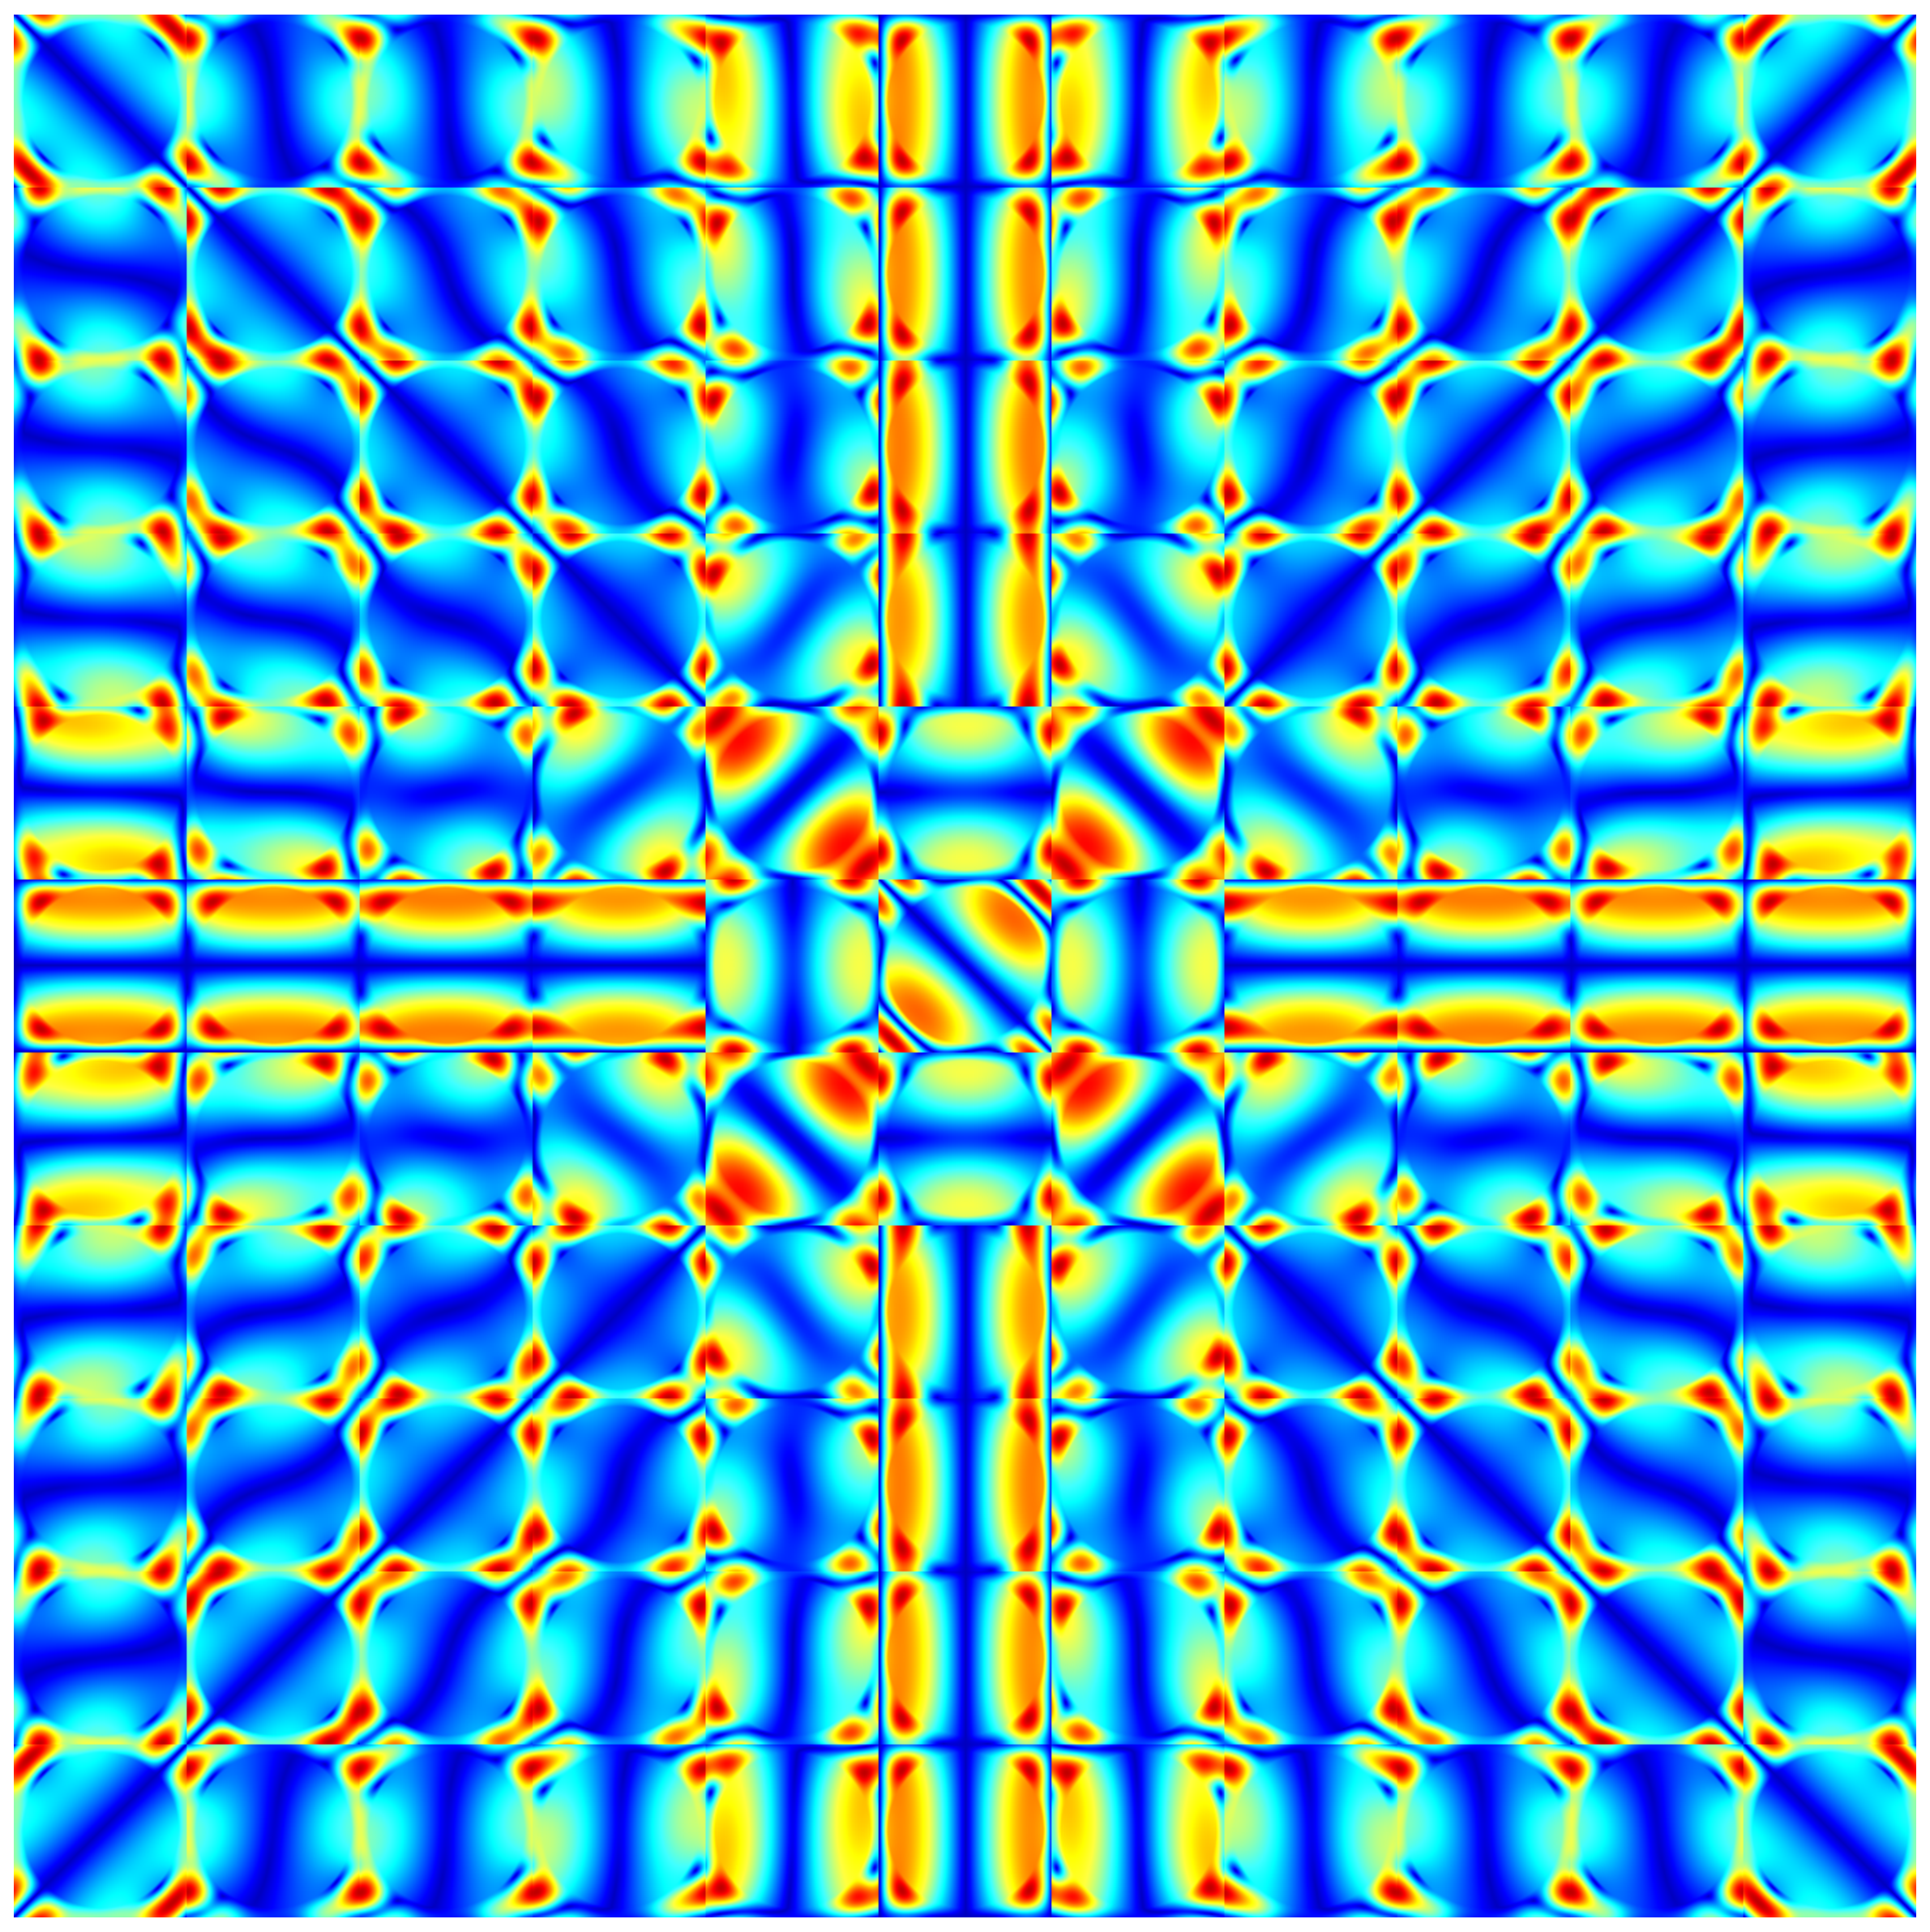
\includegraphics[width=9cm]{Titlepage/coverpicture.eps}\\
    }
    \vspace*{\stretch{8}}
    { \Large
      \color{red} Bachelor's/Master's thesis \\
      \vspace*{\stretch{0.5}}
      by \\
      \vspace*{\stretch{0.5}}
      \bf \color{red} author \\
    }
    \vspace*{\stretch{2}}
    { \large 
      \color{red} hand-in date\\
    }
    \vspace*{\stretch{5}}
    { \large
      \begin{tabular}{r@{\hspace{2em}}l}
        Instructor:     & Prof.~Dr.~J"org Schmalian\\
        2nd Instructor: & PD.~Igor~Gornyi
      \end{tabular}
    }
  \end{center}
  \vspace*{\stretch{1}}
\end{titlepage}
\cleardoublepage
 %%% if the thesis is english, add a second english titlepage
%\chapter{Acknowledgments}

I would like to express my thanks to my advisor J\"org Schmalian who encouraged and supported me and gave the right hints at the right time during the last year. 
His essential input lead to the results presented in this work. 

Furthermore, I would like to thank Una Karahasanovic for all the discussions and information which became decisive for one topic of this work. 

Then, I have to thank especially Jian Kang who crucially contributed to the discussion of bond currents and Rafael Fernandes for the fruitful discussions on the general topic. 

Special thanks to all the colleagues of the condensed matter group at the KIT. Especially to Bhilahari Jeevanesan for all the discussions and help with several problems and to Pablo Schad for finalizing this work. 

Last but not least, I have to thank my family, my mother and sister and especially Anja for all the support and encouraging words. 
 
   %%% acknowledge help from colleagues and friends 

\tableofcontents %Inhaltsverzeichnis
%\listoffigures

\pagestyle{scrheadings}			%%% for normal text, display section names in header line

\mainmatter
%%Modify overview chapter
\makeatletter% siehe De-TeX-FAQ
\renewcommand*{\chapterformat}{%
\begingroup% damit \unitlength-Änderung lokal bleibt
\setlength{\unitlength}{1mm}%
\begin{picture}(0,40)(0,5)%
\setlength{\fboxsep}{0pt}%
%\put(0,0){\framebox(20,30){}}%
%\put(0,20){\makebox(20,20){\rule{20\unitlength}{20\unitlength}}}%
\put(0,15){\color{black}\linethickness{0.4pt}\line(1,0){\dimexpr\textwidth-0\unitlength\relax\@gobble}}% line
%\put(0,0){\makebox(18,20)[r]{\fontsize{20\unitlength}{1}\color{white}\selectfont\thechapter %\kern-.04em% Ziffer in der Zeichenzelle nach rechts schieben
%}}%
\put(20,15){\makebox(\dimexpr \textwidth-20\unitlength\relax\@gobble,\ht\strutbox\@gobble)[l]{%\ %\normalsize\color{black}\chapapp~\thechapter\autodot 
}}%
\end{picture} % <- Leerzeichen ist hier beabsichtigt!
\endgroup
}%
\makeatother

\newcommand{\nocontentsline}[3]{}
\newcommand{\tocless}[2]{\bgroup\let\addcontentsline=\nocontentsline#1{#2}\egroup}

\setcounter{chapter}{-1}
\tocless\chapter{Overview}
\addcontentsline{toc}{chapter}{Overview}


%%%%%%%%%%%%%%%%%%%%%%%%%%%%%%%%%%%%%%%%%%%%%%%%%%%%%%%%%%%%
%%%%%%%%%%%%%%%%%%%%%%%%%%%%%%%%%%%%%%%%%%%%%%%%%%%%%%%%%%%%
%%%%%%%                            %%%%%%%%%%%%%%%%%%%%%%%%%
%%%%%   chapter headings             %%%%%%%%%%%%%%%%%%%%%%%
%%%%%%                             %%%%%%%%%%%%%%%%%%%%%%%%%
%%%%%%%%%%%%%%%%%%%%%%%%%%%%%%%%%%%%%%%%%%%%%%%%%%%%%%%%%%%%
%%%%%%%%%%%%%%%%%%%%%%%%%%%%%%%%%%%%%%%%%%%%%%%%%%%%%%%%%%%%

%%% INFO: when using different fonts, the chapter headings may look
%%% different and the given sizes do no longer apply!

\colorlet{chapter}{darkblue}
\addtokomafont{chapter}{\color{black}}

\makeatletter% siehe De-TeX-FAQ
\renewcommand*{\chapterformat}{%
\begingroup% damit \unitlength-Änderung lokal bleibt
\setlength{\unitlength}{1mm}%
\begin{picture}(20,40)(0,5)%
\setlength{\fboxsep}{0pt}%
%\put(0,0){\framebox(20,30){}}%
%\put(0,20){\makebox(20,20){\rule{20\unitlength}{20\unitlength}}}%
\put(20,15){\color{black}\linethickness{0.4pt}\line(1,0){\dimexpr\textwidth-20\unitlength\relax\@gobble}}% line
\put(0,0){\makebox(18,20)[r]{\fontsize{20\unitlength}{1}\color{black}\selectfont\thechapter %\kern-.04em% Ziffer in der Zeichenzelle nach rechts schieben
}}%
\put(20,15){\makebox(\dimexpr \textwidth-20\unitlength\relax\@gobble,\ht\strutbox\@gobble)[l]{%\ %\normalsize\color{black}\chapapp~\thechapter\autodot 
}}%
\end{picture} % <- Leerzeichen ist hier beabsichtigt!
\endgroup
}%
\makeatother


%\chapter{Introduction}
\label{ch:introduction}

% Zun\"achst: transport in graphene, warum cool
First successfull transport experiments in graphene \cite{Zhang2005}, \cite{Novoselov2005}

First thing that is weird about (gapless) graphene: it is described by a relativistic, massless Dirac electrons. Experiments \cite{Novoselov2005} show that electronic transport is goverened by Dirac equation, charge carriers have an effective "speed of light". This paper shows unusual effects that are characteristic for two-dimensional Dirac fermions: 1) Conductivity in graphene never falls below a minimum value (even when charge carrier density goes to zero) 2) anomalous integer quantum hall effect (occurs at half integer filling factors)
Transport measurements in graphene: integer quantum hall effect, weak localization, 

\cite{Zhu2017}: Spectra of MLG and BLG graphene are gapless and protected by symmetry of crystal lattice. When symmetry is broken by interaction with substrate or applying electric field: energy gap opens. In BLG: energy gap can be controlled by displacement field $\mathbf{D}$. Controlled induction of insulating state in graphene \cite{Oostinga2008}

\cite{Zhu2017}: Manchester group, proximity induces superconductivity: high gap energies (big gap), but still there is low resistivity (not the expected insulating state). Conductive channels were found an explained for both MLG and BLG at the Charge neutrality point and were explained by valley currents, zero energy edge states. 

supercurrent at charge neutrality point porpagates along edge channels, shunts the insulating bulk in graphene. Question adressed: in graphene, large gaps can be opened, but they rarely lead to an highly insulating state which would be expected at low temperatures. Idea: edge currents are responsible for transport, edge conductance due to nontrivial topology of gapped Dirac spectrum: 1) electronic states due to zigzag segments. 2) valley Hall effect ?
%Übergang zu Supraleitung und Fraunhofer paatern

Why study Fraunhofer patterns? By measuring critical current as a function of perpendicular B, the local current density in x direction perpendicular to current flow can be deduced \cite{Dynes1971}. By variying top and bottom voltage it is possible to keep BLG graphene charge neutral while doping the two graphene layers with the opposite sign. This results into the displacement field which translates directly into the gap.At high doping ($E_F > E_\text{gap}$, the critical current depends weakly on the displacement field.

\cite{Heersche2007}: Josephson effect in mesoscopic junctions: charge density in the graphene layer can be controlled by a gate electrode. Observation of of a supercurrent that (depending on gate voltage) is carried either by electrons in the conduction band or by holes in the valence band. finding of a finite normal state conductance and finite supercurrent at zero charge density

%Zusammenfassung: supercurrent ist geil und kann genutzt werden, um den Stromfluss zu untersuchen. Aber die Frage  ist doch eigentlich: kann man die Amplitude und das confinement gleichzeitig ver\"andern? Siehe dazu das QPC gate!


\chapter{Framework for analytical model}
\label{ch:basics}

\section{Theory of superconductivity}

The discovery of the isotope effect in 1950 revealed that not only lattice electrons but rather the whole lattice determines the superconducting properties of a solid. Experiments measuring the critical temperature $T_c$ of different mercury isotopes showed that indeed, there is a relation between the isotope mass and $T_c$. Herbert Fr\"olich was then the first to introduce a new concept to explain superconductivity. He showed that a phonon-intermediated interaction between electrons and the lattice could lead to an attractive long-range interaction of electrons in the lattice. Figuratively speaking, an electron passing through the crystal lattice will polarize it by attracting the positive ions. It leaves a deformed lattice, which will then attract a second electron. An effective attractive interaction between these two electrons is created. % – they form a Cooper pair. 
In 1956, Cooper showed that the electronic ground state, the Fermi sea at $T = 0$, is unstable if a weak attractive interaction is taken into account. This layed the foundation of the BCS theory \cite{Bardeen1957}, the first microscopic theory after the discovery in 1911 by Heike Kammerlingh Onnes. 

%TODO maybe include picture that explains, why opposite k vectors
%Cooper instability

\subsection*{Formulas needed}
Hamiltonian:
\begin{align}
H &= H_0 + H_1 \label{eq:H}\\
H_0 &= \sum_{\mathbf{k}, \sigma} \xi_{\mathbf{k}} c^{\dagger}_{\mathbf{k} \sigma }c_{\mathbf{k} \sigma }  \label{eq:H0}\\
H_1 &= \frac{1}{N} \sum_{\mathbf{k}, \mathbf{k'}} V_\mathbf{{\mathbf{k}, \mathbf{k'}}} c^{\dagger}_{\mathbf{k} \uparrow }c^{\dagger}_{- \mathbf{k} \downarrow}   c_{- \mathbf{k'} \downarrow} c_{\mathbf{k'} \uparrow} \label{eq:H1}
\end{align}
The operators $c^\dagger_{\mathbf{k}, \sigma} , c_{\mathbf{k}, \sigma}$ are fermion operators that create or annihilate an electron with momentum $\mathbf{k}$ and spin $\sigma$. The first term in the Hamiltonian $H$ is the unperturbed electron Hamiltonian $H_0$ with parabolic energy dispersion $\xi_{\mathbf{k}}$. The  second term is the interaction Hamiltonian $H_1$, expressing the scattering of two electrons from $(- \mathbf{k'} \downarrow,  \mathbf{k'} \uparrow)$ to $(\mathbf{k} \uparrow , - \mathbf{k} \downarrow)$. The interaction potential $V_\mathbf{{\mathbf{k}, \mathbf{k'}}}$ exchanges the scattering for electrons with energy $|\xi_\mathbf{k}| \lesssim \hbar \omega_D$.
%TODO check!
The Hamiltonian in eq. (\ref{eq:H}) can be simplified by doing a mean-field approximation. In this approximation, an operator $A$ is expressed by a sum of its statistical mean $\braket{A}$ and small statistical fluctuations $\delta A$. Since the fluctuations are assumed to be small, terms with $\mathcal{O}((\delta A)^2)$ can be neglected.
\begin{align}
A &= \langle A \rangle + \delta A, \quad B = \langle B \rangle + \delta B  \nonumber \\
A B &= \langle A \rangle  \langle B \rangle  + \langle A \rangle  \delta B +  \langle B \rangle \delta A + \underbrace{\delta A \delta B}_{\approx 0}\label{eq:meanfield-der}
\end{align}
Using $\delta A = A - \langle A \rangle$ and inserting this back into eq. (\ref{eq:meanfield-der}) leads to
\begin{equation}
AB = \langle A \rangle B + \langle B \rangle A - \langle A \rangle \langle B \rangle.\label{eq:meanfield-ab}
\end{equation}
This approximation is applied to the interaction part $H_1$ in eq. (\ref{eq:H1}), replacing
\begin{equation}
A = c^{\dagger}_{\mathbf{k} \uparrow }c^{\dagger}_{- \mathbf{k} \downarrow}, \quad B =  c_{- \mathbf{k'} \downarrow} c_{\mathbf{k'} \uparrow} .
\end{equation}
The result is the BCS-Hamiltonian
\begin{equation}
H_{\text{BCS}} = \sum_{\mathbf{k}, \sigma} \xi_{\mathbf{k}} c^{\dagger}_{\mathbf{k} \sigma }c_{\mathbf{k} \sigma }    -  \sum_{\mathbf{k}} \Delta_{\mathbf{k}}^* c_{-\mathbf{k}, \downarrow} c_{\mathbf{k}, \uparrow}  - \sum_{\mathbf{k}} \Delta_{\mathbf{k}}  c^{\dagger}_{\mathbf{k} \uparrow} c^{\dagger}_{- \mathbf{k} \downarrow} + \text{const.}\label{eq:H-BCS}
\end{equation}
where 
\begin{eqnarray}
\Delta_{\mathbf{k}} &:=& - \frac{1}{N} \sum_{\mathbf{k'}} V_\mathbf{{\mathbf{k} \mathbf{k'}}} \langle c_{-\mathbf{k'}, \downarrow} c_{\mathbf{k'} \uparrow} \rangle \\
\Delta_{\mathbf{k}}^* &:=& - \frac{1}{N} \sum_{\mathbf{k'}} V_\mathbf{{\mathbf{k}, \mathbf{k'}}}  \langle  c^{\dagger}_{\mathbf{k'} \uparrow} c^{\dagger}_{- \mathbf{k'} \downarrow} \rangle
\end{eqnarray}
%TODO why is this the pair potential?
The BCS-Hamiltonian in eq. (\ref{eq:H-BCS}) can be diagonalized using the Bogoliubov transformation. The aim is to express the Hamiltonian in the basis of new fermion operators. These new operators will describe quasiparticles, which are a linear combination of $c^\dagger_{\mathbf{k}, \sigma}$ and $c_{\mathbf{k}, \sigma}$.
\begin{equation}
\begin{pmatrix}
\gamma_{\mathbf{k} \uparrow} \\ \gamma^{\dagger}_{-\mathbf{k} \downarrow}  
\end{pmatrix} = \begin{pmatrix}
u^*_{\mathbf{k} } & -v_{\mathbf{k} } \\
v^*_{\mathbf{k} }  & u_{\mathbf{k} } 
\end{pmatrix} 
\begin{pmatrix}
c_{\mathbf{k} \uparrow} \\ c^{\dagger}_{-\mathbf{k} \downarrow}  
\end{pmatrix}
\end{equation}\label{eq:bogol-trans}
Evaluating the fermion anticommutation relation using the transformation above yields
\begin{equation}
\left\{ \gamma_{\mathbf{k} \uparrow}, \gamma^{\dagger}_{\mathbf{k} \uparrow}  \right\}  = \dots = |u_{\mathbf{k}}|^2 | + v_{\mathbf{k}}|^2 \stackrel{!}{=} 1
\end{equation}
and will lead to the inverse transformation of eq. (\ref{eq:bogol-trans}). Inserting the inverse transformation into the BCS-Hamiltonian in eq.(\ref{eq:H-BCS}) will give the coefficients $u_{\mathbf{k}}$, $v_{\mathbf{k}}$ from eq. (\ref{eq:bogol-trans}) and finally yield to the diagonalized form of the BCS-Hamiltonian
\begin{eqnarray}
H_{\text{BCS}} &=&  \sum_{ \mathbf{k} \sigma } E_{ \mathbf{k} } \gamma^{\dagger}_{\mathbf{k} \sigma } \gamma_{\mathbf{k} \sigma }\\
E_{\mathbf{k}} &:=&  \sqrt{\xi^2_{\mathbf{k}}  + |\Delta_{\mathbf{k}}|^2 }
\end{eqnarray}
%\begin{figure}
%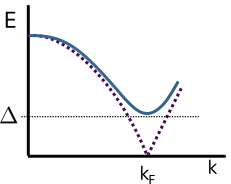
\includegraphics[width=\textwidth]{bcs-spectrum}
%\end{figure}
%TODO below:
\textbf{interpretation as holes, etc \\
plots of particle and hole exitation (dispersion relation with gap)\\
metion fermi surface and so on} \\

\subsection*{Bogoliubov de Gennes Hamiltonian}
%Motivation for BdG: Describing inhomogneous systems, example Josephson junctions --> need for a microsopic theory for inhomogenous systems. 
%Idea: make BCS- mean field hamiltonian spatially dependent. 
The ansatz for the BCS ground state used by Bardeen, Cooper and Schrieffer is based on the concept of Cooper pairs. It is a direct consequence of the instability in the ground state through the attractive interaction. The BCS theory proposes a BCS ground state built on eigenstates of the single-particle Hamiltonian $H_0$ from eq. (\ref{eq:H0}), leading to a ground state that consists of a linear combination of pair states. %TODO check!
\begin{eqnarray}
\ket{\psi_\text{BCS}} &=& \prod_{ \mathbf{k} } (u_\mathbf{k} + v_\mathbf{k} c^{\dagger}_{ \mathbf{k} \uparrow } c^{\dagger}_{ - \mathbf{k} \downarrow }) \ket{\text{vac}} \\
H_\text{BCS} \ket{\psi_\text{BCS}} &=& E_\text{BCS} \ket{\psi_\text{BCS}}  
\end{eqnarray}
In most cases however, a more realistic set-up or inhomogeneous system cannot be described in terms of eigenfunctions of $H_0$. With a vector potential $\mathbf{A} \neq 0$, for example, time reversal symmetry is not given any more. %TODO Überleitung (“In the general case”)
The characteristic length scale is the superconducting coherence length $\xi_0$. If a system is varying slowly over a length scale $l \approx \xi_0$, a spatially dependent, more general Hamiltonian is needed. 
In order to find an adequate expression for such a spatially dependent Hamiltonian, the following spinor is introduced
\begin{equation}
\ket{\Psi_\mathbf{k}} = \begin{pmatrix}
| \Psi_\mathbf{k_1} \rangle \\ | \Psi_\mathbf{k_2} \rangle
\end{pmatrix} := \begin{pmatrix}
c^{\dagger}_{\mathbf{k}, \uparrow} \\ c_{- \mathbf{k}, \downarrow}
\end{pmatrix} \ket{\psi_\text{BCS}} \label{eq:spinor}
\end{equation}
In this basis $\left\{| \Psi_\mathbf{k_1} \rangle, | \Psi_\mathbf{k_2} \rangle \right\}$, the Hamiltonian is (and this is the Bogoliubov de Gennes Hamiltonian with energies relative to $E_\mathbf{k}$):
\begin{equation}
H_\text{BdG}\left(\mathbf{k} \right) = \begin{pmatrix}
\xi_\mathbf{k} &  - \Delta_\mathbf{k}\\
- \Delta^*_\mathbf{k} & - \xi_\mathbf{k}
\end{pmatrix} \label{eq:H-BdG}
\end{equation}
%For this, the commutation relation for $H_\text{BCS}$ and $c^\dagger_{\mathbf{k}, \uparrow}$, $c_{- \mathbf{k}, \downarrow}$ have been used.
This Hamiltonian form eq. (\ref{eq:H-BdG}) has the eigenvalues
\begin{equation}
 \pm E_\mathbf{k} = \pm \sqrt{\xi_\mathbf{k}^2 + |\Delta_\mathbf{k}|^2  }.
\end{equation}
%Include eigenstates?
To finally arrive at the spatially dependent form of eg. (\ref{eq:H-BdG}), the Hamiltonian is Fourier-transformed.
\begin{eqnarray}
H_\text{BdG} \left( \mathbf{r} \right) &:=& \frac{1}{N} \sum_\mathbf{k} e^{i \mathbf{k \cdot r}} H_\text{BdG}\left( \mathbf{k} \right) \\
&=& \begin{pmatrix}
H_0\left( \mathbf{r} \right)  &  - \Delta \left( \mathbf{r} \right) \\
- \Delta^* \left( \mathbf{r} \right)  & - H_0 \left( \mathbf{r} \right) 
\end{pmatrix} \label{eq:H-BdG-r}
\end{eqnarray}
$H_0 \left( \mathbf{r} \right) $ is the free Hamiltonian. Corresponding Schr\"odinger equaions are called BdG-equations:
\begin{eqnarray}
H_\text{BdG} \left( \mathbf{r} \right) \Psi\left( \mathbf{r} \right) &=& E \Psi\left( \mathbf{r} \right)\label{eq:BdG-eq} \\
\Psi\left( \mathbf{r} \right)  &=& \begin{pmatrix}
\Psi_1\left( \mathbf{r} \right) \\ \Psi_2\left( \mathbf{r} \right) 
\end{pmatrix}\label{eq:BdG-spinor}
\end{eqnarray}

\section{Andreev reflection- NS interface}\label{sec:NS}

Now that the principles of BCS theory have been established, the physical effects at the interface between a superconductor and a normal are to be outlined.\\
The most important detail when modelling the interface between a superconductor and a normal metal is the superconducting order parameter $\Delta \left( \mathbf{r} \right)$. It is present in the superconducting region and zero in a normal metal. To keep the model as simple as possible, a step-like behaviour is assumed. This means that for an interface placed at $x=0$, the superconducting order parameter becomes a function of $x$ and can be written as
\begin{equation}
\Delta \left( x \right) = \theta \left(x \right)\label{eq:delta }
\end{equation}.
How does this model differ from a quantum mechanical step potential set-up? The formalism is virtually identical, but there is a subtle and important difference in the results. In the normal region, there are electrons, whereas in the superconducting regions, there is a condensate of Cooper pairs. A normal electron can be reflected at the interface as a hole and an additional Cooper pair can be created in the superconducting region.\\
By solving the Bogoliubov-de-Gennes equation in (\ref{eq:BdG-eq}), this picture becomes clearer.  This equation needs to be solved both for the normal and the superconducting region. When treating this problem quantum-mechanically, energies below and above the gap need to be considered independently. The resulting wave functions have to be continuous at the interface. Depending on the region, the gap parameter in the Hamiltonian in eq. (\ref{eq:H-BdG-r}) is either zero or $\Delta_0$.

\subsection*{Semi-classical approximation: Andreev equations}

In case of the NS interface, the gap parameter varies slowly over scales of $k_F$, and it may vary over scales of the coherence length $\xi_0$. Because $k_F$ is a good length scale for this problem, the equations above can be simplified:
\begin{equation}
\begin{pmatrix} u \\ v \end{pmatrix} = e^{i \mathbf{k_F} \mathbf{r} } \begin{pmatrix} U (x) \\ V(x) \end{pmatrix}.
\end{equation}
Since $U(x)$ and $V(x)$ vary slowly over distances of order $k_F^{-1}$, the second derivative can be neglected. This is the semi-classical approximation, which then leads to the Andreev equations
\begin{eqnarray}
- i \hbar \mathbf{v}_F \nabla U + \Delta V &=& \epsilon U \\
 i \hbar \mathbf{v}_F \nabla V + \Delta^* U &=& \epsilon V.
\end{eqnarray}
These equations are significantly easier to handle than the BdG-equations, since they describe a first-order problem.
\newline
\newline
Consider an incoming particle from the left half-space $x < 0 $, travelling towards the superconducting interface at $x=0$, assuming that both the normal region and the superconductor have the same Fermi velocity $k_F^{-1}$. The one-dimensional Andreev equations for the NS interface read
\begin{eqnarray}
- i \hbar v_{F, x} \frac{d}{dx} U + \Delta(x) V &=& \epsilon U \\
 i \hbar v_{F, x} \frac{d}{dx} V + \Delta^*(x) U &=& \epsilon V.
\end{eqnarray}

\subsubsection*{Solution for the normal region}
In the normal region (for $x < 0$) the superconducting gap parameter decreases to zero on a length scale shorter than $\xi$. Therefore, the step-like approximation from eq. (\ref{eq:delta }) holds. In the normal region, 
the coefficients $U(x)$ and $V(x)$ are independent. The ansatz contains an incident wave with unity amplitude and a reflected hole with amplitude $a$. 
\begin{equation}
\begin{pmatrix} U(x) \\ V(x) \end{pmatrix}_N = e^{i k_N x } \begin{pmatrix} 1 \\ 0 \end{pmatrix} + a e^{-i k_N x } \begin{pmatrix} 0 \\ 1 \end{pmatrix} 
\end{equation}
where 
\begin{equation}
k_n = \frac{\epsilon}{\hbar v_x}
\end{equation}
And therefore the solution to the Andreev reflection is ($|\mathbf{k}| = k_F$)
\begin{eqnarray}
\begin{pmatrix} u \\v \end{pmatrix} &=& e^{i\mathbf{k} \cdot \mathbf{r}} \begin{pmatrix} U(x) \\V(x) \end{pmatrix}\\
&=& e^{i\mathbf{q}_+ \cdot \mathbf{r}} \begin{pmatrix} 1 \\ 0\end{pmatrix} + a e^{i\mathbf{q}_- \cdot \mathbf{r}} \begin{pmatrix} 0 \\ 1\end{pmatrix},
\end{eqnarray}
with
\begin{equation}
\mathbf{q}_\pm =  \left( k \pm \frac{\epsilon}{\hbar v_F} \right) \hat{\mathbf{k}} 
\end{equation}

\subsubsection*{Solution in the superconducting region}
In the superconducting region, the solution for the wave function has the form
\begin{equation}
\begin{pmatrix} U(x) \\ V(x) \end{pmatrix}_S = c e^{i k_S x } \begin{pmatrix} U_0 \\ V_0 \end{pmatrix},
\end{equation}
where $c$ is the amplitude and $k_S$ is the wave vector. The expression for $k_S$ depends on the energy of the incoming particle, which can be either \emph{above} or \emph{below} the gap.\newline \newline
For high energies \emph{above} the gap,  $E > |\Delta|$ , the wave vector is
\begin{equation}
k_S = \frac{\sqrt{\epsilon^2 - \Delta^2}}{\hbar v_x}
\end{equation}
The coherence factor $U_0$, $V_0$ can be found by solving the BdG equations within the BCS framework. Matching the boundary conditions at the interface yields
\begin{equation}
a = \frac{V_0}{U_0}, \quad c = \frac{1}{U_0}.
\end{equation}
In this solution, the incoming electron has the momentum 
\begin{equation}
q  = k_F + \frac{\epsilon}{\hbar v_F} \quad \rightarrow \epsilon(q) = \hbar v_F \left( q - k_F \right)
\end{equation}
with a positive group velocity $v_g = v_F$, whereas the reflected hole has the momentum
\begin{equation}
q  = k_F - \frac{\epsilon}{\hbar v_F} \quad \rightarrow \epsilon(q) = \hbar v_F \left( k_F - q \right)
\end{equation} 
with negative group velocity $v_g = - v_F$. \\
By calculating the change in the momentum one finds the trajectory of the reflected hole to coincide with the trajectory of the incoming electron. The change in momentum is
\begin{equation}
\Delta p_x = \left( \hbar k_x - \frac{\epsilon}{v_x} \right) -  \left( \hbar k_x + \frac{\epsilon}{v_x} \right) = - \frac{2 e }{v_x}
\end{equation}
$p_y$, $p_z$ are conserved, $\Delta p_x$ is small, therefore the trajectory of the reflected hole is almost the same as the trajectory of the incoming electron.
%TODO figure!
%Probabilities: 
%\begin{equation}
%|a|^2 + (U_0^2- V_0^2)|c|^2 = 1
%\end{equation}
\newline
\newline
For energies \emph{below} the gap, $\epsilon < |\Delta |$, there are no states available inside the gap, therefore the wave function decays inside the superconductor. 
\begin{equation}
\tilde{k}_S= \frac{\sqrt{\Delta^2 - \epsilon^2 }}{\hbar v_x}.
\end{equation}
The wave function is
\begin{equation}
\begin{pmatrix} U(x) \\ V(x) \end{pmatrix}_S = c e^{- \tilde{k_S} x } \begin{pmatrix} U_0 \\ V_0 \end{pmatrix}.
\end{equation}
For sub-gap energies, the amplitudes of the normal wave functions are slightly modified:
\begin{equation}
a = \frac{\tilde{V_0}}{\tilde{U_0}}, \quad c = \frac{1}{\tilde{U_0}}
\end{equation}
and 
\begin{equation}
\tilde{U_0} = \frac{1}{\sqrt{2}} \left( 1 + i \frac{\sqrt{|\Delta|^2 - \epsilon^2}}{\epsilon} \right), \quad \tilde{V_0} = \frac{1}{\sqrt{2}} \left( 1 - i \frac{\sqrt{|\Delta|^2 - \epsilon^2}}{\epsilon} \right).
\end{equation}
In this case, it holds that
\begin{equation}
|a|^2 = 1
\end{equation}
In other words, there are no transmitted particles and all particles are Andreev reflected.

\section{Theory of SNS junction}
So far, only NS interfaces have been considered. The same procedure can be applied to superconductor - normal metal - superconductor (SNS) junctions: A sandwich structure of a superconductor on the left side, a normal region in the middle and a superconductor on the right side. At both interfaces, a particle can be Andreev-reflected.
Each time an electron is Andreev reflected at the right side and a hole travels back, a cooper pair is induced into the right superconductor. In the same manner, a cooper pair is stolen from the left superconductor when the hole is Andreev reflected as an electron. As an overall consequence, a supercurrent through the SNS junction can be observed. This process leads to localized electrons with bound states, the so called Andreev bound states. \\

A SNS junction with normal region at $|x| < W/2$, the right superconductor at $x > + W/2$ and the left superconductor at $x < -W/2$ is considered. The electrons in both superconducting regions and in the normal metal have the same Fermi velocity and there are no insulating barriers between them. This means that $W$  is smaller than the electron mean free path. For short $W$ this implies that the mean free path is larger than the superconducting coherence length (?). The phase difference between the superconductors is $\chi$, so the right supercondctor has phase $\chi/2$ and the left has $-\chi/2$. 
The semi classical approximation is used and a wave function with the form
\begin{equation}
\begin{pmatrix} u \\ v \end{pmatrix} = e^{i \mathbf{k_F} \mathbf{r} } \begin{pmatrix} U (x) \\ V(x) \end{pmatrix}.
\end{equation}
is needed.\newline
In the normal region, it holds that 
\begin{equation}
\begin{pmatrix} U(x) \\ V(x) \end{pmatrix}_N = A\cdot \left[ e^{i k_N x } \begin{pmatrix} 1 \\ 0 \end{pmatrix} + a e^{-i k_N x } \begin{pmatrix} 0 \\ 1 \end{pmatrix} \right], \quad k_N = \frac{\epsilon}{\hbar v_x}.
\end{equation}
Assuming that $k_x > 0$, the wave function in the right superconductor ($x > W/2$) is
\begin{equation}
\begin{pmatrix} U(x) \\ V(x) \end{pmatrix}_R = d_1 e^{ - \tilde{k}_S x } \begin{pmatrix} \tilde{U} e^{i \chi/4} \\ \tilde{V} e^{-i \chi/4} \end{pmatrix}, \quad \tilde{k}_S  = \frac{\sqrt{|\Delta|^2 - \epsilon^2 }}{\hbar |v_x|}.
\end{equation}
For the left superconductor, the wave function is
\begin{equation}
\begin{pmatrix} U(x) \\ V(x) \end{pmatrix}_L = d_1' e^{ \tilde{k}_S x } \begin{pmatrix} \tilde{V} e^{-i \chi / 4}\\ \tilde{U} e^{i \chi / 4} \end{pmatrix}.
\end{equation}
Applying the continuity condition at the interfaces leads to
\begin{eqnarray}
a e^{-i k_n W} &=& \frac{\tilde{V}}{\tilde{U}} e^{-i \chi /2}  \\
a e^{i k_n W} &=& \frac{\tilde{U}}{\tilde{V}} e^{i \chi /2}.
\end{eqnarray}
Combining these equations, we find
\begin{equation}
e^{2i ( k_N W - \chi /2 )}  = \frac{\epsilon + i \sqrt{|\Delta|^2 - \epsilon^2 }}{ \epsilon - i \sqrt{|\Delta|^2 - \epsilon^2 } } \label{eq:energy-exp}.
\end{equation}
To simplify this expression, one can introduce 
\begin{equation}
\sin \alpha := \frac{\epsilon}{|\Delta|}, \quad - \pi / 2 < \alpha < \pi / 2\label{eq:sinalpha}
\end{equation}
Using eq. (\ref{eq:sinalpha}), one can rewrite the right hand side of eq. (\ref{eq:energy-exp}) in terms of trigonometric functions and gets
\begin{equation}
e^{2i ( k_N W - \chi /2 )} = e^{-2i \alpha + i \pi},
\end{equation}
which then leads to
\begin{equation}
\epsilon = \frac{\hbar v_x}{W} \left( \pi \left(l + \frac{1}{2} \right) - \arcsin \frac{\epsilon}{|\Delta|} + \frac{\chi}{2} \right).
\end{equation}
%TODO short summary, what has been done up to this point?
If $k_x < 0 $, it holds that
\begin{equation}
\begin{pmatrix} U(x) \\ V(x) \end{pmatrix}_R = d_2 e^{ - \tilde{k}_S x } \begin{pmatrix} \tilde{V} e^{i \chi/4} \\ \tilde{U} e^{-i \chi/4} \end{pmatrix}
\end{equation}
For the left superconductor, the wave function is
\begin{equation}
\begin{pmatrix} U(x) \\ V(x) \end{pmatrix}_L = d_2' e^{ \tilde{k}_S x } \begin{pmatrix} \tilde{U} e^{-i \chi / 4}\\ \tilde{V} e^{i \chi / 4} \end{pmatrix}
\end{equation}
An analogous calculation leads to
\begin{equation}
\epsilon = - \frac{\hbar |v_x|}{W} \left( \pi \left(l - \frac{1}{2} \right) + \arcsin \frac{\epsilon}{|\Delta|} + \frac{\chi}{2} \right)
\end{equation}
The final result for the spectrum is
\begin{equation}
\epsilon = \pm \frac{\hbar |v_x|}{W} \left( \pi \left(l \pm \frac{1}{2} \right) \mp \arcsin \frac{\epsilon}{|\Delta|} + \frac{\chi}{2} \right)
\end{equation}
The upper sign is equivalent to $k_x > 0$ and the lower sign is equivalent to $k_x  <0 $.\\
Normalizing the wave functions yields the coefficient
\begin{equation}
|A|^2 = \frac{1}{2(W+ k_S^{-1})} = \frac{1}{2} \frac{\sqrt{|\Delta|^2 - \epsilon^2}}{\hbar |v_x| + W \sqrt{|\Delta|^2 - \epsilon^2}}.
\end{equation}
%TODO maybe a bit more how |A|^2 is calculated?
\subsubsection*{Limit of short junction}

For junctions with small width $W$,
\begin{equation}
W \ll \frac{\hbar v_x }{|\Delta|}, \quad \xi \ll W
\end{equation}
where $\xi \sim \hbar v_F / |\Delta|$ is the coherence length. Then, in eq. (\ref{eq:energy-exp}) the term with $e^{2i k_n W} \approx 1$ and the spectrum becomes
\begin{equation}
\epsilon = \mp \cos \frac{\chi}{2}, \quad 0 < \chi < \pi
\end{equation}

\subsubsection*{Limit of long junction}

Long junction, $W \gg \xi_0$, it hold that 
\begin{equation}
W \gg \frac{\hbar |v_x|}{|\Delta|} 
\end{equation} 
then the spectrum is (because $\arcsin \frac{\epsilon}{|\Delta|}$ can be neglected
\begin{equation}
\epsilon = \pm \frac{\hbar |v_x|}{W}\left(\frac{\chi}{2} - \frac{\pi}{2} \right) + \frac{l \pi \hbar |v_x|}{W} 
\end{equation}

\section{Supercurrent through the SNS junction}
Having established the normal wave functions for SNS junctions, the quantum-mechanical current can be calculated.
\begin{equation}
\mathbf{j} = \frac{e}{m} \left[ f_n u_n^* \left( \mathbf{r} \right) \left( - i \hbar \nabla - \frac{e}{c} \mathbf{A} \right) u_n\left( \mathbf{r} \right) + \left(1-f_n\right) v_n\left( \mathbf{r} \right) \left( -i \hbar \nabla - \frac{e}{c} \mathbf{A} \right) v_n^*\left( \mathbf{r} \right) + \text{c.c.} \right] \label{eq:current-qm}
\end{equation}
$n$ labels quantum states, $f_n$ is the corresponding Fermi distribution.
As a simplification, $\mathbf{A} = 0$ is considered. For evaluating eq. (\ref{eq:current-qm}), the normal wave functions are used. In the semi-classical approximation, only the derivatives of the rapidly varying functions $e^{i\mathbf{k r}}$ contribute to the current.
\begin{eqnarray}
\mathbf{j} &=& - i \hbar  \frac{e}{m} \left[ f_n u_n^* \left( \mathbf{r} \right) \nabla  u_n \left( \mathbf{r} \right) + \left(1-f_n\right) v_n\left( \mathbf{r} \right) \nabla v_n^*\left( \mathbf{r} \right) + \text{c.c.} \right]\\
I_x &=& - \frac{e}{\hbar} \sum_n \left(1- 2 f_n \right) \frac{\hbar v_x \sqrt{|\Delta^2| - \epsilon_n^2}}{\hbar v_x + W \sqrt{|\Delta|^2 -\epsilon^2}}
\end{eqnarray}

\section{Specular Andreev reflection, graphene specifics}
An unusual form of Andreev reflection has been found on graphene - superconductor interfaces %TODO cite.
In the previously discussed Andreev retro reflection, the electron and the reflected hole both lie in the conductance band. In more exotic materials, like  single layer graphene (SLG), the reflected hole undergoes a transition to the valence band. In this case, the reflection angle is a function of $E_F$, and for $E_F = 0$, the reflection is specular.
For graphene, the single particle Hamiltonian is the Dirac Hamiltonian
\begin{eqnarray}
H &=& \begin{pmatrix}
H_+ & 0 \\
0 & H_- 
\end{pmatrix} \\
H_\pm &=& i \hbar \left( \sigma_x \delta_x \pm \sigma_y \delta_y \right) + U
\end{eqnarray}
This modifies the BdG-equation and leads to interesting results when calculating the Andreev reflection amplitude. 
\begin{equation}
\begin{pmatrix}
H_\pm + E_F & \Delta \\
\Delta^* & E_F - H_\pm 
\end{pmatrix} \begin{pmatrix}
u \\ v \end{pmatrix} = \epsilon \begin{pmatrix} u \\v \end{pmatrix} \label{eq:dirac-hamiltonian}
\end{equation}
The electron spinor has two components $\begin{pmatrix} u_1, u_2\end{pmatrix} = \begin{pmatrix} \Psi_{A+}, \Psi_{B+} \end{pmatrix}$, and the hole spinor is $\begin{pmatrix} v_1, v_2\end{pmatrix} = \begin{pmatrix} \Psi^{*}_{A-} - \Psi^{*}_{B-} \end{pmatrix}$.
The Hamiltonian from eq. (\ref{eq:dirac-hamiltonian}) leads to the energy spectrum
\begin{equation}
\epsilon = \sqrt{|\Delta|^2 + \left( E_F - U \pm \hbar v |\mathbf{k}|\right) ^2}, \quad |\mathbf{k}| = \sqrt{k_x^2 + k_y^2}.
\end{equation}
The dispersion relation has four solutions for $\mathbf{k}$. Since $k_y$ and $\epsilon$ are preserved, a general scattering state is a superposition of these four solutions for $k_x$. The derivative $\hbar^{-1} d\epsilon / d k_x$, the velocity in x direction, gives two solutions with negative slope and two with positive slope. The two solutions for $k_x$ which lead to a positive velocity consist of one electron excitation ($v=0$) and one hole excitation ($u=0$). 
From the BCS mean field theory it is known that $\Delta_0 \ll E_F + U_0$, or equivalently $\xi = \hbar v /\Delta_0 \gg \lambda_F^{sc}$, the Fermi wave length in the superconductor. The magnitude of $\xi$ and the Fermi wave length in the normal region, $\lambda_F^{n}$, is not constrained.
%TODO pretty picture
%TODO 
Look at the solution for two different regimes:\\
$\mathbf{\epsilon < E_F}$:  the reflected hole is in an empty state in the conduction band. A conduction band hole moves opposite to its wave vector, so $v_y$, $v_x$ change sign $\rightarrow$ Andreev retro reflection \\
$\mathbf{\epsilon > E_F}$: reflected hole is in an empty state in the valence band. Valence band hole moves into same direction as its wave vector, so $v_y$ remains the same, $v_x$ changes sign $\rightarrow$ Andreev specular reflection. \\
At energies $\epsilon \lesssim \Delta_0$, retro reflection is the dominant process for $E_F \gg \Delta_0$, and specular reflection dominates if $E_F \ll \Delta_0$.
The probability of the electron--hole conversion can be calculated by solving the Dirac-BdG equations matching boundary conditions at the interface. The resulting reflection amplitude for electron to electron (what) is denoted with $r\left( \epsilon, \alpha\right)$, where $\alpha$ is the angle of incidence (angle between incoming vector and x-axis). The Andreev reflection amplitude for electron to hole is $r_A \left( \epsilon, \alpha \right)$. The difference of the NS interface for graphene and a superconductor is that the Andreev reflection amplitude is unity for $\alpha = 0$, whereas in a normal NS interface Andreev reflection is suppressed for all angles. 
The fact that the reflection at the interface always converses the charge is a consequence of the conservation of chirality, meaning the sublattice index. When an electron is Andreev reflected as a hole, the reflected hole moves on the same sublattice, while the reflection without charge conversion would require scattering from one sublattice to the other. (?)

% Specular reflection manifests itself in the differential conductance


%Applying the same methods as above, the 
 


%\chapter{Analytical Model}
\label{ch:analyticalmodel}
\textit{This chapter intends to explain the calculation of the critical current in different SNS junctions. For this purpose, a quasiclassical transport theory is used and its foundations are explained in the first section. This technique is then employed for a clean SNS junction and an expression for the Josephson current is found. In the following section the calculations used for the clean setup are extended for the more sophisticated quantum point contact (QPC) and here as well, the current for the QPC-gated junction is found.}

\section{Foundation of the quasiclassical model}
This section explains preliminary assumptions made to describe the current in a SNS junction. The aim is to express the current through the junction using a quasiclassical approach. Essentially, this means that the Andreev bound states are associated with straight trajectories connecting the superconducting leads. The superconducting current density is then expressed in terms of these trajectories.\\
\begin{figure}[h]
\centering	
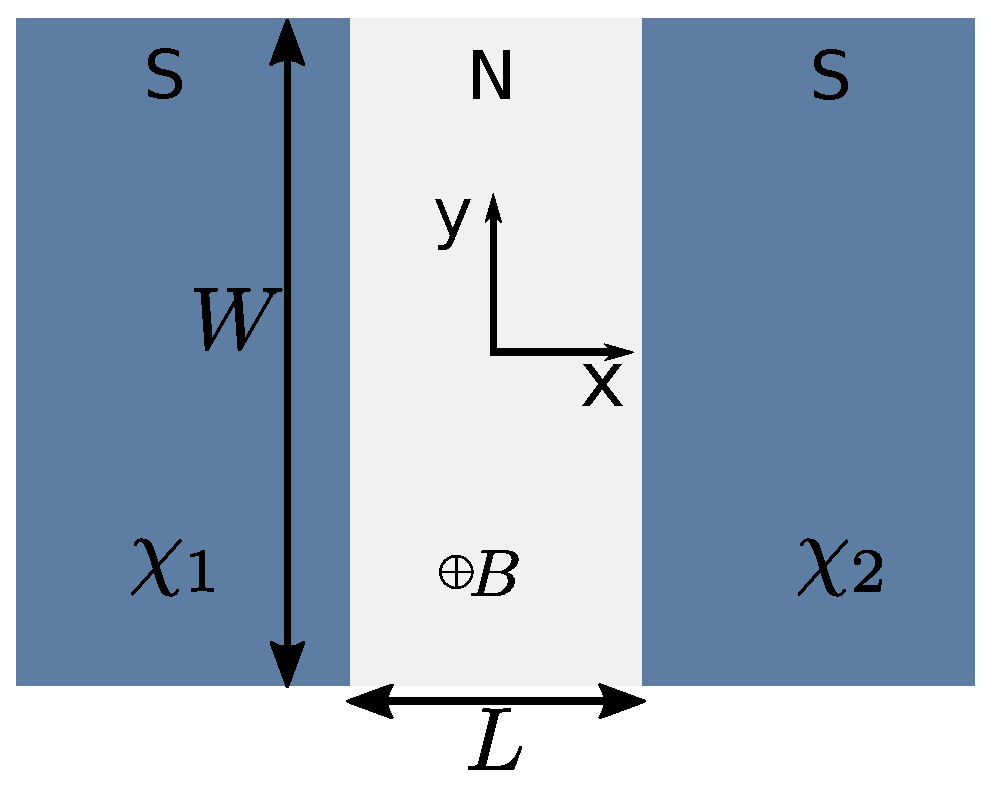
\includegraphics[width=0.6\textwidth]{figure/analyticalmodel/sns_junction}
\caption{Schematic representation of a short and wide SNS junction.}
\label{fig:sns_schematic}
\end{figure}

The two dimensional junction, a schematic is shown in fig \ref{fig:sns_schematic}, is a short and wide junction with width $W$ and length $L$, where $W \gg L$. The NS-interfaces are parallel to the $y$-axis and are placed at $x = \pm L/2$. Each of the superconducting leads has a phase $\chi_{1}$ and $\chi_{2}$ and the overall phase difference is $\chi = \chi_{1} - \chi_{2}$. The superconducting gap parameter is only present in the superconducting leads and zero in the normal region and can be expressed as
\begin{equation}
\Delta\left( x \right) = |\Delta| e^{\chi_1} \Theta\left(-L/2 -x \right) + |\Delta| e^{\chi_2} \Theta\left(x-L/2 \right) 
\label{eq:gap_parameter}
\end{equation}
We consider the low temperature limit, where the thermal length scale of the system is smaller larger than the sample length:
\begin{equation}
L_T = \hbar v_F / k_B T \gg L
\end{equation}
The considered sample is ballistic, the fermi wavelength $\lambda_F$ is smaller than the sample length $L$. It has the BCS coherence length $\zeta = \hbar v_F / \pi \Delta$, where $\zeta$ is much larger than the Fermi velocity $\zeta \gg v_F$ 
\textbf{TODO: (in order to induce superconductivity in the system?)}. 
The relation between the coherence length $\zeta$ and the sample length $L$ determines, if the considered junction is a \textit{short} or a \textit{long} junction:
\begin{eqnarray*}
\zeta \ll L \quad \rightarrow \quad \text{long junction} \quad \rightarrow \quad \text{many Andreev levels} \\ 
\zeta \gg L \quad \rightarrow \quad \text{short junction} \quad \rightarrow \quad \text{one Andreev level} 
\end{eqnarray*}
\textbf{TODO: replace equation above with good picture (E < delta, andreec levels...)}\\
%TODO stimmt das oben? Es sollte einen Zusammenhang primaer mit Energie, nicht mit sample size geben...
The presence of magnetic field in the normal region of the sample will lead to a bending of the trajectories due to the Lorentz force. Depending on the strength of magnetic field $B$ and the Fermi velocity the radius of this curve is 
\begin{equation}
r_B = \frac{m^* v_F}{e B}
\end{equation}
%TODO check if correct!
In order to justify the assumption of straight trajectories, either the magnetic field has to be weak enough or the Fermi velocity (wavelength) has to be large (short) enough. Then, the cyclotron radius $r_B$ is larger than the sample size $L$ and straight trajectories are a valid assumption. 

\section{Plane setup: calculation of current}
%TODO Re-calculate current from Glazman
To derive the current for the SNS setup depicted in figure \ref{fig:sns_schematic}, we start by writing down the Bogoliubov-de-Gennes Hamiltonian for this system.
\begin{equation}
\begin{pmatrix}
-\frac{\hbar^2}{2m} \nabla^2 - \epsilon_F & \Delta(x) \\
\Delta^*(x) & \frac{\hbar^2}{2m} \nabla^2 + \epsilon_F 
\end{pmatrix}
\begin{pmatrix}
\psi_e \\
\psi_h
\end{pmatrix} = E 
\begin{pmatrix}
\psi_e\\
\psi_h
\end{pmatrix}
\end{equation}
The Hamiltonian above uses eq. (\ref{eq:gap_parameter}) for the spatially dependent superconducting gap parameter $\Delta(x)$. The eigenvalue problem has two solutions
\begin{equation}
\epsilon_{\pm} = \frac{\hbar^2 k^2_{\pm}}{2m} = -\epsilon_F - \sqrt{E_k^2 - |\Delta|^2}
\end{equation}
%The corresponding wavefunction (according to Glazman paper):
%\begin{equation}
%\psi_e^{n, \pm} = \frac{1}{\sqrt[WL]{}}
%\end{equation}
%TODO calculate current and wavefunctionsx
\textbf{TODO: Hier fehlt die Herleitung f\"ur Wellenfunktionen, Ausdruck f\"ur den Strom etc.!}
Current density for short and long junction limit: 
In the short junction limit the current density can be derived from the scattering matrix formalism and it reads
\begin{equation}
\mathcal{J}^s (\chi) = \frac{\mathcal{T} \sin \chi}{\sqrt{1 - \mathcal{T} \sin^2 \frac{\chi}{2}}}
\end{equation}
$\mathcal{T}$ is the transmission coefficient that describes the transmission through a channel (each channel corresponds to a eigenvalue of the scattering matrix.
The current density for the long junction limit is
\begin{equation}
\mathcal{J}(\chi) = \sum_{k = 1}^{\infty} \frac{(-1)^{k+1}}{k} \sin( k \chi).
\end{equation}
\begin{figure}
\centering
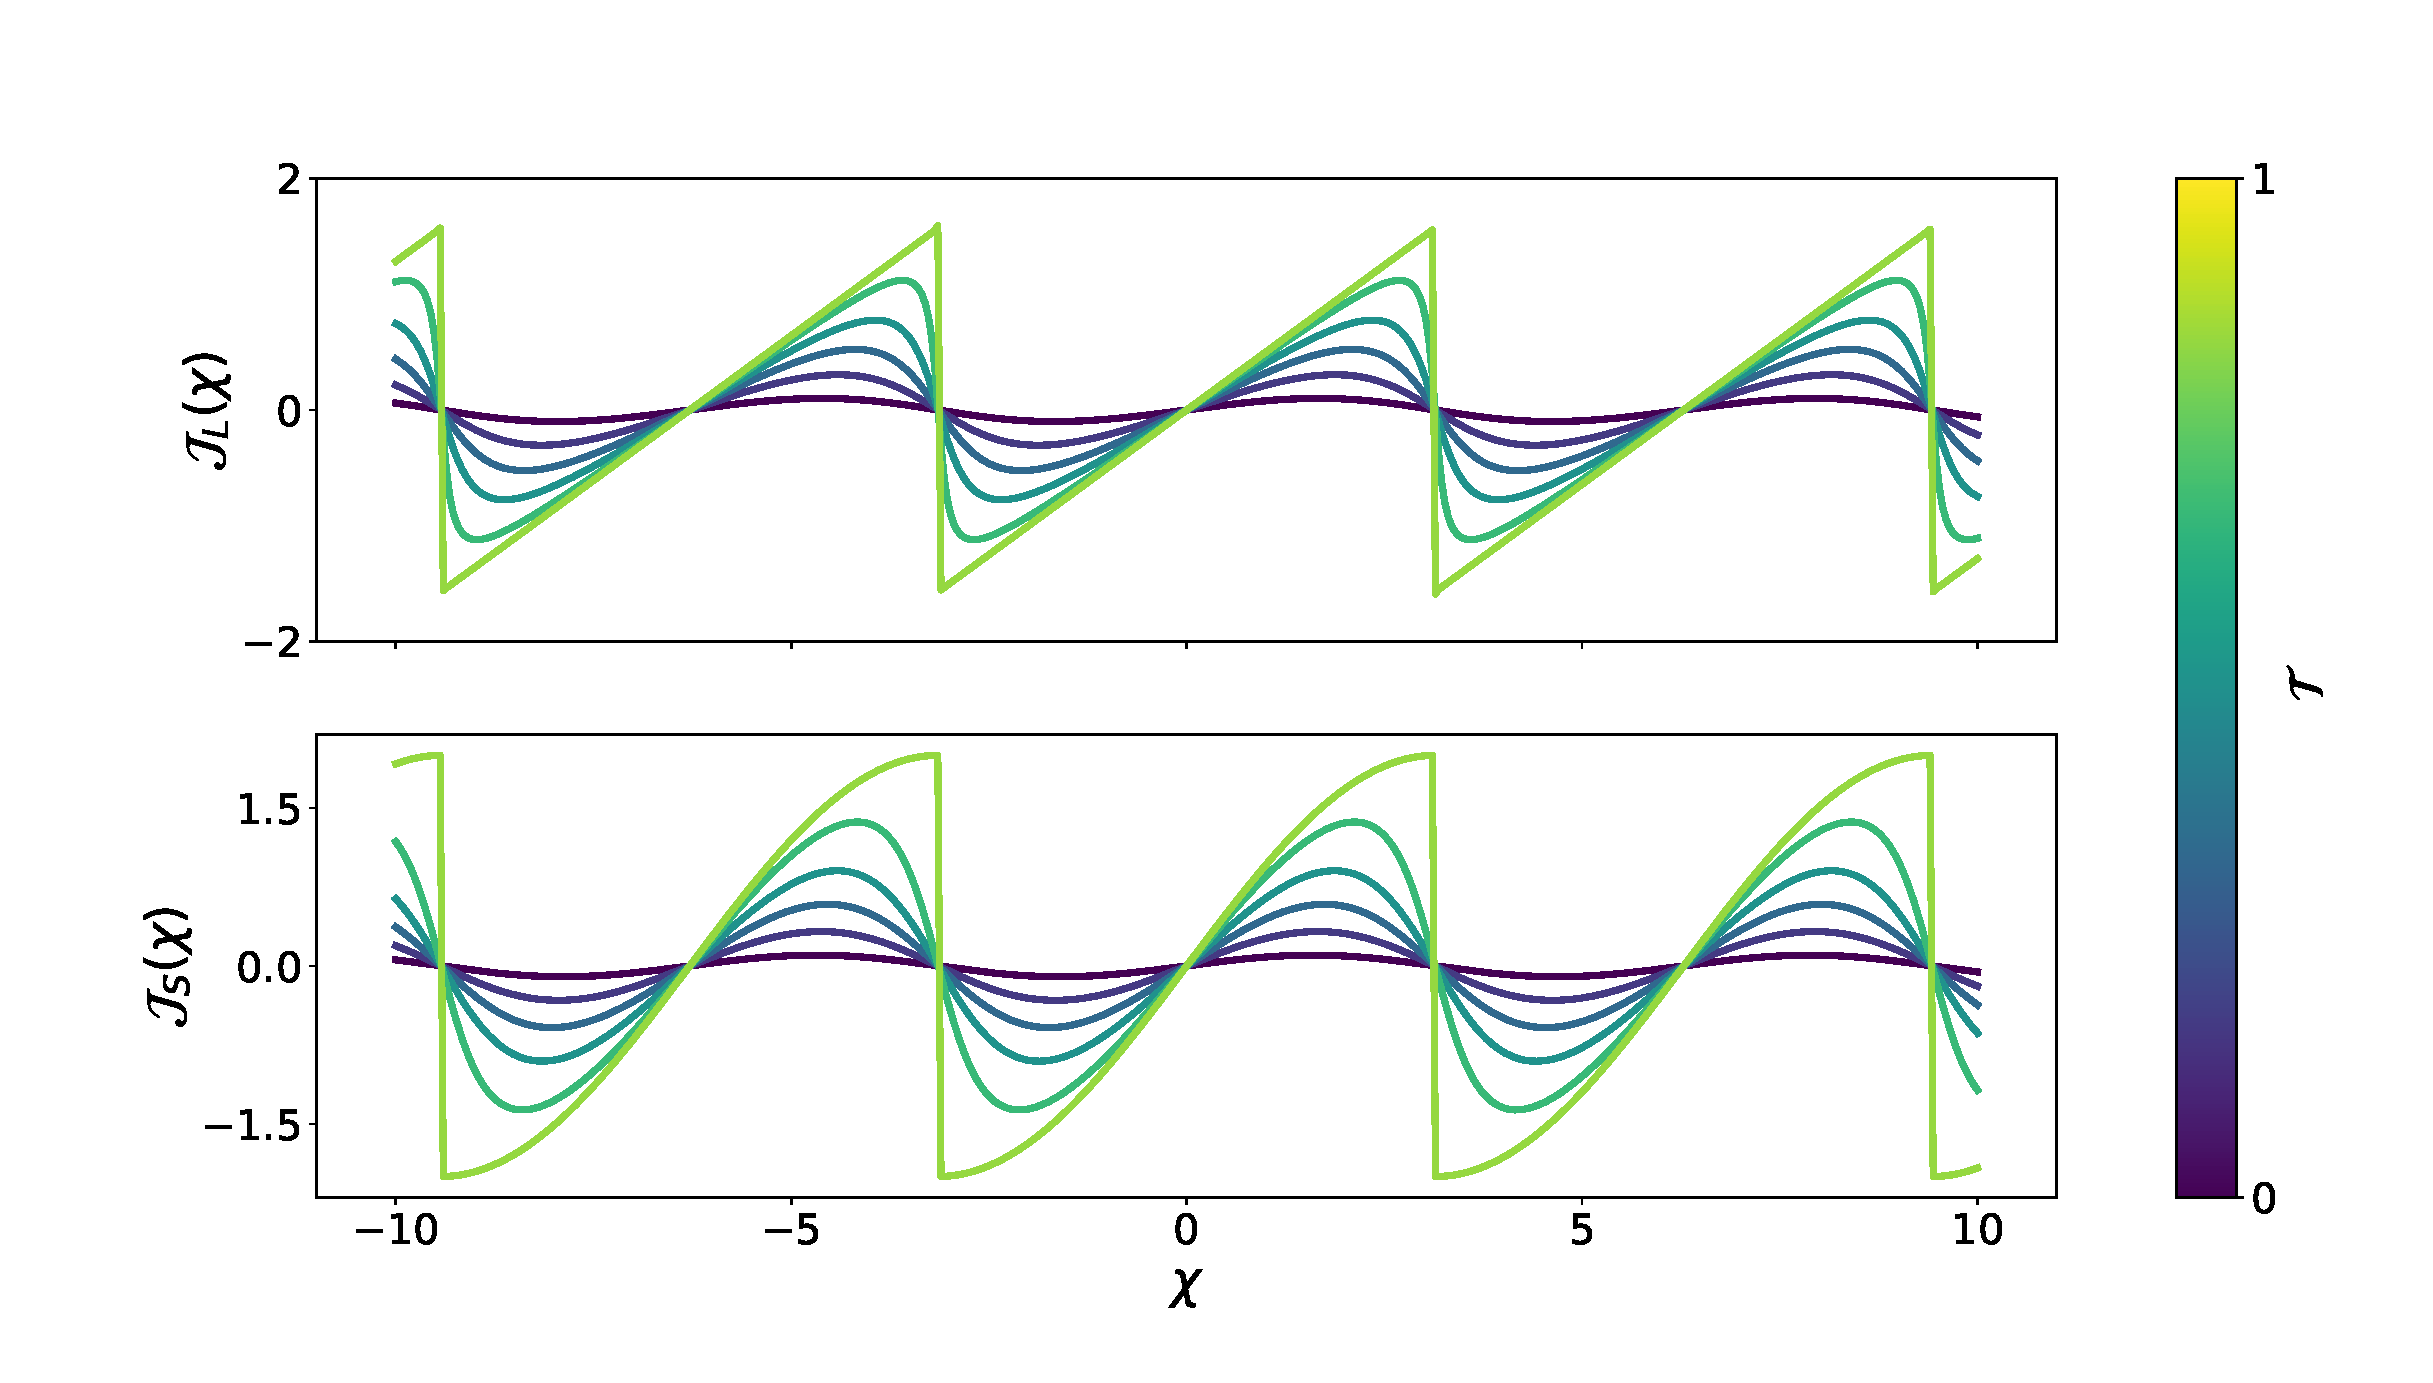
\includegraphics[width=\textwidth]{figure/analyticalmodel/current_density_all}
\caption{Short and long junction current density}
\label{fig:current_density}
\end{figure}
Figure \ref{fig:current_density} shows a plot of both short and long junction limit current densities. They differ for a large transmission coefficient $\mathcal{T} \simeq 1$, where in the long junction limit we observe a sawtooth like shape and in the short junction limit we have a sinusoidal shape.\\
Using the current density the Josephson current at zero magnetic field ($\phi = 0$) can be expressed as 
\begin{equation}
J\left(\chi, \phi=0\right) = \frac{2 e v_F}{\pi \lambda_F L^2}  \int \int_{-W/2}^{W/2} d y_1 d y_2 \frac{\mathcal{J}(\chi)}{\left[ 1 + \left(\frac{y_1 - y_2}{L}\right)^2\right]^2}
\label{eq:josephson_current_zero_b}
\end{equation}
\subsection*{Including magnetic field}
So far, the current has been derived for zero magnetic field. If a finite magnetic field is considered, the phase $\chi$ will be modified because of two effects. The magnetic phase that will be acquired along a trajectory connecting two points $y_1$ and $y_2$  leads to an additional term in the phase. Then again, \textit{the condition of zero screening current in the bulk superconducting region and the limit of} $\lambda_L \rightarrow 0$ \textit{require the superconducting phase at the interfaces to become functions of y} \textbf{TODO: ? Umschreiben!}.\\
Assuming that the London penetration depth is small to zero in the superconducting regions the following gauge for the vector potential can be used
\begin{equation}
\mathbf{A}=A_y \mathbf{e}_y, \quad
A_y=\left\{ 
		\begin{array}{ll}
				-B x, & -L/2 \leq x \leq L/2, \\[0.2cm] 
				-\frac{1}{2} B L |x| , & \quad |x|>L/2
		\end{array} 
	\right.
\label{eq:Ay}
\end{equation}
The gauge in eq. (\ref{eq:Ay}) will give no additional contribution to the phase on straight trajectories
\begin{eqnarray}
\delta \chi &=& \frac{2 \pi}{\Phi_0} \int d \mathbf{l} \cdot \mathbf{A} \\
&=& \frac{2 \pi}{\Phi_0} \int_{-L/2}^{L/2} \frac{dx}{\cos \theta} A_y (x) \sin \theta \\
&=& - \frac{2 \pi B}{\Phi_0} \frac{y_2 - y_1}{L} \int_{-L/2}^{L/2} x dx \\
&=& 0
\end{eqnarray}
and therefore, the only contribution to the magnetic phase is
\begin{equation}
\delta \chi = -\frac{\pi \phi (y_1 + y_2)}{W} \quad \Leftrightarrow \quad \tilde{\chi}(y_1, y_2) = \chi  -\frac{\pi \phi (y_1 + y_2)}{W}.
\label{eq:chi_plane}
\end{equation}
This mean that the current phase relation in the expression for the Josephson current from eq. (\ref{eq:josephson_current_zero_b}) for zero magnetic field has to replaced by the effective phase $\chi \rightarrow \tilde{\chi}(y_1, y_2)$ and then reads
\begin{equation}
J\left(\chi, \phi \right) = \frac{2 e v_F}{\pi \lambda_F L^2}  \int \int_{-W/2}^{W/2} d y_1 d y_2 \frac{\mathcal{J}(\tilde{\chi}(y_1, y_2))}{\left[ 1 + \left(\frac{y_1 - y_2}{L}\right)^2\right]^2}
\label{eq:josephson_current}
\end{equation}
By maximizing the Josephson current with respect to $\chi$, the critical current can be found:
\begin{equation}
I_c(\phi) = \text{max}_{\chi}\left\{ J(\chi, \phi) \right\}
\end{equation}
\textbf{Dependence on W/L ratio? Plot of current?}

\section{Calculation of QPC current}
\begin{figure}
\centering
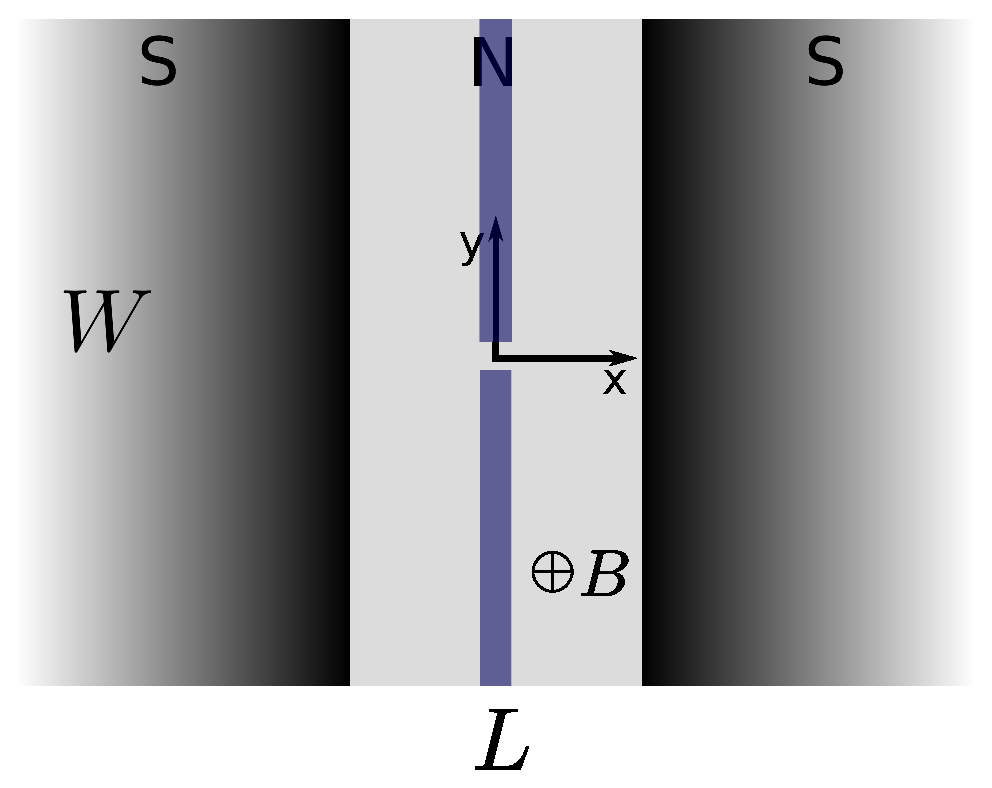
\includegraphics[width=0.6\textwidth]{figure/analyticalmodel/qpc_sns_junction}
\caption{QPC setup.}
\label{fig:qpc_sns_schematic}
\end{figure}
\textbf{TODO: what happens when a constriction is on top of normal layer, fermi levels etc}
The quasiclassical formalism can even be employed to modified SNS junctions. One can build gates on top of the normal region of the junction in a way that the current cannot pass through the gated regions. In the quasiclassical picture this means that the possibilites for trajectories connecting two points at the superconducting interfaces are limited through the geometry of the constriction.\\
Figure \ref{fig:qpc_sns_schematic} shows a schematic of the quantum point contact setup which will be analysed with the quasiclassical formalism. The normal region of the SNS junction is covered by a gate in the middle that has a small split in the middle. The split is located at $(x y) = (0, 0)$ so that the sample is symmetric around the origin. The width of the split is in the order of $\lambda_F$ (\textbf{Warum wichtig?}) and can thereby be modelled as an isotropic scattering point with transmission coefficient $\mathcal{T}_0$. Consequently, each trajectory connecting the two superconducting interfaces have to pass through the QPC. For simplicity the geometrical width of the barrier is neglected and only straight trajectories (no scattering at side edges) are considered. This modified setup leads first to a different parametrisation of the trajectories and therefore to a different magnetic phase than in eq. (\ref{eq:chi_plane}).\\
With the QPC setup, all possible trajectories are parametrised by two angles $\theta_i$ and $\theta_f$. $\theta_i$ describes the trajectory before passing through the QPC in the region $ -L/2 < x 0$ and  $\theta_f$ after passing through the QPC. The parametrisation of the trajectories reads
\begin{equation}
\tan \theta_i = - \frac{2 y_i}{L}, \quad \tan \theta_f = \frac{2 y_f}{L}
\end{equation}
With the gauge from eq. (\ref{eq:Ay}) the magnetic phase acquired within the sample reads:
\begin{eqnarray}
\frac{2\pi}{\Phi_0} \int d\mathbf{l} \cdot \mathbf{A}  &=&
-\frac{\pi B}{\Phi_0}\left(\frac{L}{2}\right)^2
\left(-\tan\theta_i + \tan\theta_f\right) =
-\frac{\pi \phi (y_i+y_f)}{2 W}.
\label{eq:phaseQPC}
\end{eqnarray}
Therefore the effective phase is
\begin{equation}
\tilde{\chi}(y_i,y_f)=\chi-\frac{3\pi \phi }{2W}(y_i+y_f).
\label{eq:chiQPC}
\end{equation}
The effective phase for the QPC in eq. (\ref{eq:chiQPC}) is half of to the effective phase without any constriction, in eq. (\ref{eq:chi_plane}). This seems reasonable, since in the QPC setup the all possible straigth trajectories can cover only half of the normal region compared to the setup without constriction.
The effective phase therefore modifies the current phase relation $\mathcal{J}(\tilde{chi}(y_i, y_f)$. Beyond that, the expression for the critical current has to be modified as well.

The normalized critical current reads
\begin{eqnarray}
\frac{I_c(\phi)}{I_c(0)} &=& \frac{ \text{max}_{\chi} \int d \theta_i \cos^2 \theta_i\int d \theta_f \cos \theta_f \mathcal{J}(\tilde{\chi}(\theta_i, \theta_f)) }{ \text{max}_{\chi} \int d \theta_i \cos^2 \theta_i\int d \theta_f \cos \theta_f \mathcal{J}(\chi) }
\end{eqnarray}
In the limit of small transmission probability $\mathcal{T} << 1$ we use Eq.~(\ref{sawT<1}) for the partial Josephson current. The normalized critical current can then be written as 
\begin{eqnarray}
\frac{I_c(\phi)}{I_c(0)} &=& \frac{\mathcal{I}_2(\phi)\mathcal{I}_{3/2}(\phi)}{\mathcal{I}_2(0)\mathcal{I}_{3/2}(0)}
\end{eqnarray}
The integrals $\mathcal{I}$ are here defined as
\begin{equation}
\mathcal{I}_k(\phi) = \frac{2}{L}\int_{-W/2}^{+W/2}dy \frac{\cos\left(\frac{3\pi\phi y}{2W}\right)}{\left[1 + \left(\frac{2y}{L}\right)^2 \right]^k}
\label{integral-qpc}
\end{equation}
At $\phi=0$ we get
\begin{equation}
\mathcal{I}_2(0)\mathcal{I}_{3/2}(0) =
\frac{L}{\sqrt{L^2+W^2}}\arctan\frac{W}{L} + \frac{L^2W}{(L^2+W^2)^{3/2}}
\label{Ic-0}
\end{equation}
The parabolic asymptotics of the critical current at small $\phi$ is found by expanding
the cosine factors in the numerator:
\begin{eqnarray}
\frac{I_c(\phi)}{I_{c0}}&\simeq& 1 - \frac{9\pi ^2 \phi^2 }{32} f_0(W/L) \\
f_0(x) &=& \frac{\sqrt{x^2+1} \log \left(\sqrt{x^2+1}+x\right)}{x}- \frac{x}{x+\left(x^2+1\right) \arctan(x)} 
\end{eqnarray}
In the opposite limit of high fields, $\phi\to \infty$, we extend the integration in Eq.~(\ref{integral-qpc}) over $y_i$ and $y_f$ to $\pm \infty$ and obtain
\begin{eqnarray}
\frac{I_c(\phi)}{I_{c0}} &\simeq& \frac{\pi^3 }{8x^2}\left(\frac{3\phi}{2x}\right)^{3/2}\frac{\left(1+x^2\right)^{3/2}}{x + \left(1+x^2\right)\arctan x}\exp\left(-\frac{3\phi\pi}{2x}\right)
\label{large-phi}
\end{eqnarray}
change in magnetic phase, geometrical argument, change in current, limits etc. 

%TODO wie weiter?
%Skizze erklären, wie ist das QPC aufgebaut?
%Was ändert sich für den Strom? 
%Wie sieht das Ergebnis aus?





%\chapter{Conclusion And Outlook}
\label{ch:conclusion}
%%%%%%%%%%%%%%%%%%%%%%%%%%%%
%Zusammenfassung der Arbeit%
%%%%%%%%%%%%%%%%%%%%%%%%%%%%

%Meine Arbeit hat sich mit SNS junctions und der quasiklassischen Beschreibung beschäftigt. Ein weiterer Punkt ist die numerische Simulation von konkreten Experimenten. Ich konnte zeigen, dass die Ergebnisse von meiner


%%%%%%%%%%%%%%%%%%%%%%%%%%%%
%		Ergebnisse?		   %
%%%%%%%%%%%%%%%%%%%%%%%%%%%%
%Es wurden Ansätze für den Transport überprüft und auf den konkreten Fall des QPC übertragen (neu entwickelt, Formel). Dieser Ansatz ist anders als in Glazman, Zagoskin etc.
%Die quasiklassische Transporttheorie wurde erfolgreich auf das QPC Setup angewendet. Es konnte gezeigt werden, dass sowohl das Limit phi -> unendlich als auch phi-> 0 korrekt wiedergegeben werden. Weiterhin konnte gezeigt werden, dass das Verhalten der Kantenströme gut beschrieben werden kann.

%Auf das Experiment eingehen, was wird gut beschrieben, was nicht? Was steht 

%Eine Berechung der kritischen Stroms im Rahmen der Streumatrix-Theorie wurde implementiert. Die Tendenz ist, dass die QPC und HB Experimente richtig wiedergegeben werden. Das Waveguide Setup konnte simuliert werden, daraus konnte, weil es der tolle Fall mit translationsinvariantem System ist, die Stromdichte mit der Dyson Fuller Methode berechnet werden. 

%%%%%%%%%%%%%%%%%%%%%%%%%%%%
%		 Ausblick		   %
%%%%%%%%%%%%%%%%%%%%%%%%%%%%

%Analytische Rechnungen können für weitere Setups berechnet werden, für kompliziertere Setups. Dabei kann beispielsweise Mehrfachstreuung und Anisotrope Streeuung hinzugezogen werden. 

%Im Kontext auf die Experimente sind die Möglichkeiten beinahe unbeschränkt. Es gibt Ansätze, für Spin Orbit Coupling in BLG, die nutzen und afwändige experimentelle Setups beschreiben.





%\listoftodos

\cleardoublepage
\addcontentsline{toc}{chapter}{Bibliography}
\bibliography{literature} 

%\begin{appendix}                         %%% start the appendix for longer calculations/info
%	\chapter{Appendix}
%\end{appendix}

\backmatter
\end{document}
